\chapter{Random Forests}\label{ch:forest}

\begin{remark}{Outline}
In this chapter, we present the well-known family of \textit{random forests}
methods. In Section~\ref{sec:4:bias-variance}, we first describe the bias-variance
decomposition of the prediction error and then present, in
Section~\ref{sec:4:ensemble}, how aggregating randomized models through
ensembles reduces the prediction error by decreasing the variance term in this
decomposition. In Section~\ref{sec:4:random-forests}, we revisit random forests
and its variants and study how randomness introduced into the decision trees
reduces prediction errors by decorrelating the decision
trees in the ensemble. Properties and features of random forests are then outlined
in Section~\ref{sec:4:features} while their consistency
is finally explored in Section~\ref{sec:4:consistency}.
\end{remark}


\section{Bias-variance decomposition}
\label{sec:4:bias-variance}

In section~\ref{sec:2:performance-evaluation}, we defined the generalization
error of a model $\varphi_{\cal L}$ as its expected prediction error
according to some loss function $L$
\begin{equation}\label{eqn:4:generalization-error}
Err(\varphi_{\cal L}) = \mathbb{E}_{X,Y} \{ L(Y, \varphi_{\cal L}(X)) \}.
\end{equation}
Similarly, the expected prediction error of $\varphi_{\cal L}$ at $X=\mathbf{x}$
can be expressed as
\begin{equation}
Err(\varphi_{\cal L}(\mathbf{x})) = \mathbb{E}_{Y|X=\mathbf{x}} \{ L(Y, \varphi_{\cal L}(\mathbf{x})) \}.\label{eqn:4:generalization-error:x}
\end{equation}

In regression, for the squared error loss, this latter form of the expected
prediction error additively decomposes into bias and variance terms which
together constitute a very useful framework for diagnosing the prediction error
of a model. In classification, for the zero-one loss, a similar decomposition
is more difficult to obtain. Yet, the concepts of bias and variance can be
transposed in several ways to classification, thereby providing comparable
frameworks for studying the prediction error of classifiers.


\subsection{Regression}
\label{sec:bias-variance:regression}

In regression, assuming that $L$ is the squared error loss, the expected
prediction error of a model $\varphi_{\cal L}$ at a given point $X=\mathbf{x}$
can be rewritten with respect to the Bayes model $\varphi_B$:
\begin{align}
& Err(\varphi_{\cal L}(\mathbf{x})) \nonumber \\
&= \mathbb{E}_{Y|X=\mathbf{x}} \{ (Y - \varphi_{\cal L}(\mathbf{x}))^2 \} \nonumber \\
&= \mathbb{E}_{Y|X=\mathbf{x}} \{ (Y -\varphi_B(\mathbf{x}) + \varphi_B(\mathbf{x}) - \varphi_{\cal L}(\mathbf{x}))^2 \} \nonumber \\
&= \mathbb{E}_{Y|X=\mathbf{x}} \{ (Y -\varphi_B(\mathbf{x}))^2  \} + \mathbb{E}_{Y|X=\mathbf{x}} \{ (\varphi_B(\mathbf{x}) - \varphi_{\cal L}(\mathbf{x}))^2 \} \nonumber \\
& \hookrightarrow + \mathbb{E}_{Y|X=\mathbf{x}} \{ 2 (Y - \varphi_B(\mathbf{x}))(\varphi_B(\mathbf{x}) - \varphi_{\cal L}(\mathbf{x})) \} \nonumber \\
&= \mathbb{E}_{Y|X=\mathbf{x}} \{ (Y -\varphi_B(\mathbf{x}))^2 \} + \mathbb{E}_{Y|X=\mathbf{x}} \{ (\varphi_B(\mathbf{x}) - \varphi_{\cal L}(\mathbf{x}))^2 \} \nonumber \\
&= Err(\varphi_B(\mathbf{x})) +  (\varphi_B(\mathbf{x}) - \varphi_{\cal L}(\mathbf{x}))^2 \label{eqn:4:decomp1}
\end{align}
since $\mathbb{E}_{Y|X=\mathbf{x}} \{ Y - \varphi_B(\mathbf{x}) \} =
\mathbb{E}_{Y|X=\mathbf{x}} \{ Y \} - \varphi_B(\mathbf{x}) = 0$ by definition
of the Bayes model in regression. In this form, the first term in the last
expression of Equation~\ref{eqn:4:decomp1} corresponds to the (irreducible)
residual error  at $X=\mathbf{x}$ while the second term represents the
discrepancy of $\varphi_{\cal L}$ from the Bayes model. The farther from the
Bayes model, the more sub-optimal the model and the larger the error.

If we further assume that the learning set ${\cal L}$ is itself a random
variable (sampled from the population $\Omega$) and that the learning algorithm is deterministic, then the expected
discrepancy over ${\cal L}$ with the Bayes model can further be re-expressed in terms of the
average prediction $\mathbb{E}_{\cal L} \{ \varphi_{\cal L}(\mathbf{x}) \}$
over the models learned from all possible learning sets of size $N$:
\begin{align}
& \mathbb{E}_{\cal L} \{ (\varphi_B(\mathbf{x}) - \varphi_{\cal L}(\mathbf{x}))^2 \}\nonumber \\
&= \mathbb{E}_{\cal L} \{ (\varphi_B(\mathbf{x}) - \mathbb{E}_{\cal L} \{ \varphi_{\cal L}(\mathbf{x}) \} + \mathbb{E}_{\cal L} \{ \varphi_{\cal L}(\mathbf{x}) \} - \varphi_{\cal L}(\mathbf{x}))^2 \} \nonumber \\
&= \mathbb{E}_{\cal L} \{ (\varphi_B(\mathbf{x}) - \mathbb{E}_{\cal L} \{ \varphi_{\cal L}(\mathbf{x}) \} )^2 \} + \mathbb{E}_{\cal L} \{ (\mathbb{E}_{\cal L} \{ \varphi_{\cal L}(\mathbf{x}) \} - \varphi_{\cal L}(\mathbf{x}))^2 \} \}\nonumber \\
& \hookrightarrow+ \mathbb{E}_{\cal L} \{ 2(\varphi_B(\mathbf{x}) - \mathbb{E}_{\cal L} \{ \varphi_{\cal L}(\mathbf{x}) \})(\mathbb{E}_{\cal L} \{ \varphi_{\cal L}(\mathbf{x}) \} - \varphi_{\cal L}(\mathbf{x}))\} \nonumber \\
&= \mathbb{E}_{\cal L} \{ (\varphi_B(\mathbf{x}) - \mathbb{E}_{\cal L} \{ \varphi_{\cal L}(\mathbf{x}) \} )^2 \} + \mathbb{E}_{\cal L} \{ (\mathbb{E}_{\cal L} \{ \varphi_{\cal L}(\mathbf{x}) \} - \varphi_{\cal L}(\mathbf{x}))^2 \} \}\nonumber \\
&= (\varphi_B(\mathbf{x}) - \mathbb{E}_{\cal L} \{ \varphi_{\cal L}(\mathbf{x}) \} )^2 + \mathbb{E}_{\cal L} \{ (\mathbb{E}_{\cal L} \{ \varphi_{\cal L}(\mathbf{x}) \} - \varphi_{\cal L}(\mathbf{x}))^2 \}
\end{align}
since $\mathbb{E}_{\cal L}\{ \mathbb{E}_{\cal L} \{ \varphi_{\cal
L}(\mathbf{x}) \} - \varphi_{\cal L}(\mathbf{x}) \} =  \mathbb{E}_{\cal L} \{
\varphi_{\cal L}(\mathbf{x}) \} -  \mathbb{E}_{\cal L} \{ \varphi_{\cal
L}(\mathbf{x}) \} = 0$. In summary, the expected generalization error additively
decomposes as formulated in Theorem~\ref{thm:bias-variance}.

\begin{theorem}\label{thm:bias-variance}
For the squared error loss, the bias-variance decomposition of the expected
generalization error $\mathbb{E}_{\cal L} \{ Err(\varphi_{\cal L}(\mathbf{x}))
\}$ at $X=\mathbf{x}$ is
\begin{equation}
\mathbb{E}_{\cal L} \{ Err(\varphi_{\cal L}(\mathbf{x})) \} = \text{noise}(\mathbf{x}) + \text{bias}^2(\mathbf{x}) + \text{var}(\mathbf{x}),
\end{equation}
where
\begin{align*}
\text{noise}(\mathbf{x}) &= Err(\varphi_B(\mathbf{x})), \\
\text{bias}^2(\mathbf{x}) &= (\varphi_B(\mathbf{x}) - \mathbb{E}_{\cal L} \{ \varphi_{\cal L}(\mathbf{x}) \} )^2, \\
\text{var}(\mathbf{x}) &= \mathbb{E}_{\cal L} \{ (\mathbb{E}_{\cal L} \{ \varphi_{\cal L}(\mathbf{x}) \} - \varphi_{\cal L}(\mathbf{x}))^2 \}.
\end{align*}
\end{theorem}

This bias-variance decomposition of the generalization error is due to
\citet{geman:1992} and was first proposed in the context of neural networks.
The first term, $\text{noise}(\mathbf{x})$, is the residual error. It is
entirely independent of both the learning algorithm and the learning set and
provides for any model a theoretical lower bound on its generalization error.
The second term, $\text{bias}^2(\mathbf{x})$, measures the discrepancy between
the average prediction and the prediction of the Bayes model. Finally, the
third term, $\text{var}(\mathbf{x})$, measures the variability of the
predictions at $X=\mathbf{x}$ over the models learned from all possible
learning sets. All three terms are illustrated in Figure~\ref{fig:bias-variance}
for a toy and artificial regression problem. Both $\text{noise}(\mathbf{x})$ and
$\text{var}(\mathbf{x})$ measures the spread of the two densities while
$\text{bias}^2(\mathbf{x})$ is the distance between their means.

\begin{figure}
    \centering
    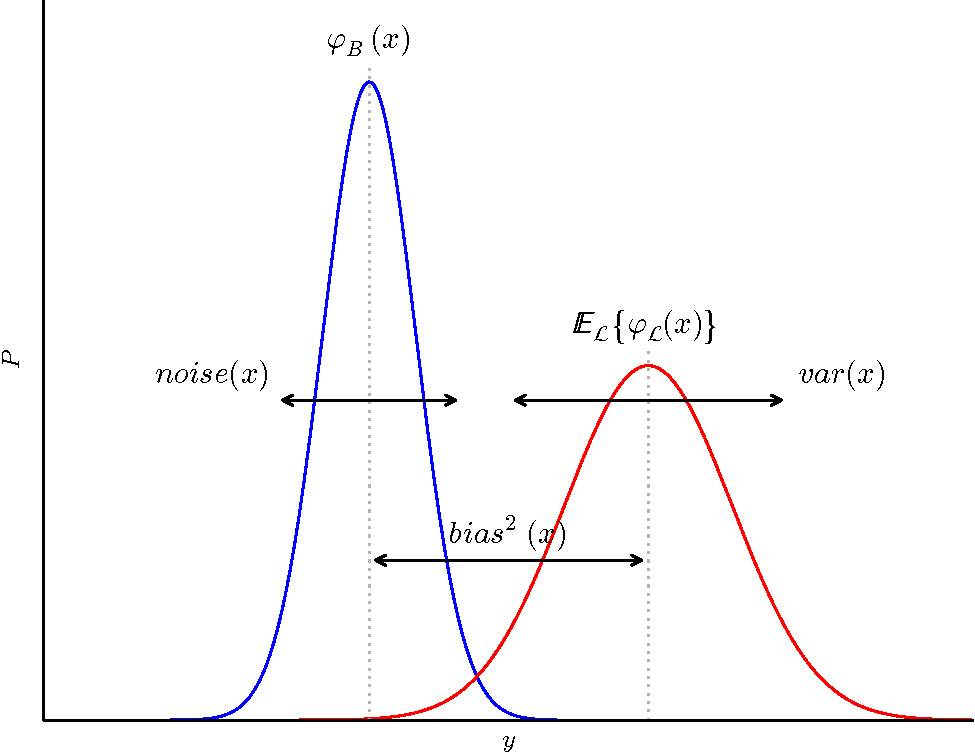
\includegraphics[width=0.9\textwidth]{figures/ch4_bias_variance.pdf}
    \caption{Residual error, bias and variance at $X=\mathbf{x}$. (Figure inspired from \citep{geurts:2002}.)}
    \label{fig:bias-variance}
\end{figure}

As a typical example, the bias-variance decomposition framework can be used as
a tool for diagnosing underfitting and overfitting (as previously introduced in
Section \ref{sec:2:model-selection}). The upper plots in
Figure~\ref{fig:overfitting} illustrate in light red predictions $\varphi_{\cal
L}(\mathbf{x})$ for polynomials of degree $1$, $5$ and $15$ learned over random
learning sets ${\cal L}$ sampled from a noisy cosine function. Predictions
$\mathbb{E}_{\cal L} \{ \varphi_{\cal L}(\mathbf{x}) \}$ of the average model
are represented by the thick red lines. Predictions for the model learned over
the learning set, represented by the blue dots, are represented in gray.
Predictions of the Bayes model are shown by blue lines and coincide with the unnoised
cosine function that defines the regression problem. The lower plots in the
figure illustrate the bias-variance decomposition of the expected
generalization error of the polynomials.

\begin{figure}
    \hspace{-0.75cm}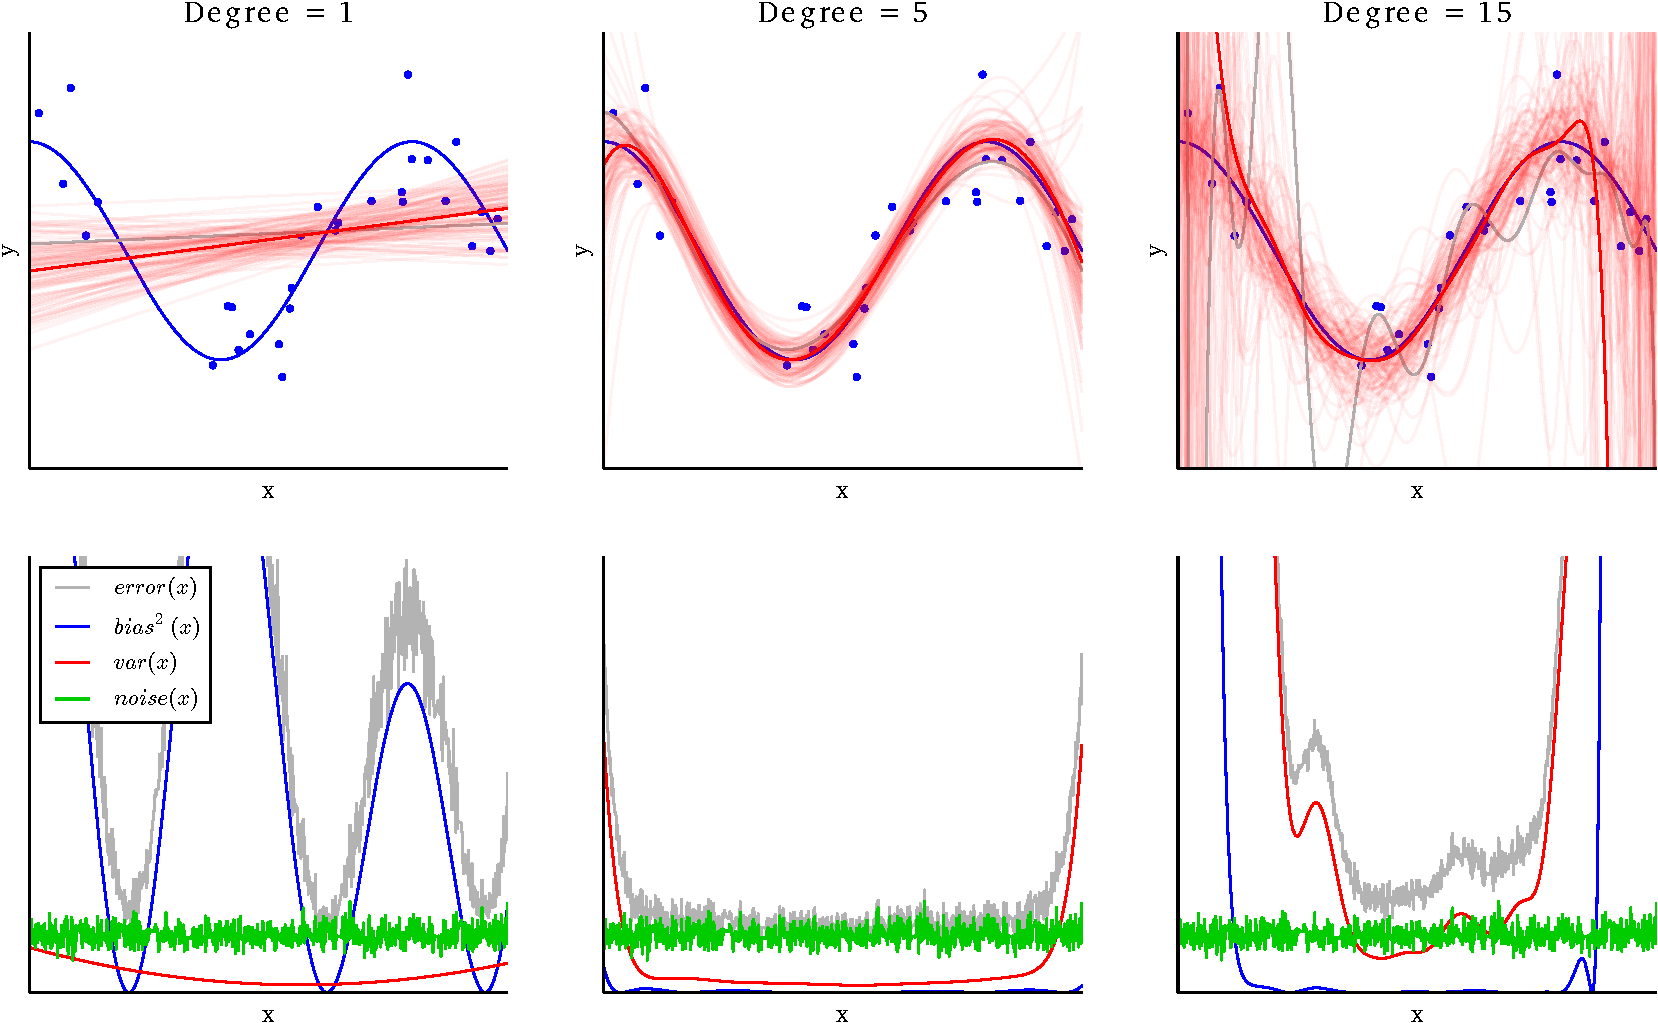
\includegraphics[width=1.1\textwidth]{figures/ch4_overfitting.pdf}
    \caption{Bias-variance decomposition of the expected generalization error for polynomials of degree $1$, $5$ and $15$.}
    \label{fig:overfitting}
\end{figure}

Clearly, polynomials of degree $1$ (left) suffer from underfitting. In terms of
bias and variance, this translates into low variance but high bias as shown in
the lower left plot of Figure~\ref{fig:overfitting}. Indeed, due to the low
degree of the polynomials (i.e., due to the low model complexity), the
resulting models are almost all identical and  the variability of the
predictions from one model to another is therefore quite low. Also, because of
low complexity, none of them really fits the trend of the training points, even
approximately, which implies that the average model is far from approximating
the Bayes model. This results in high bias. On the other hand, polynomials of
degree $15$ (right) suffer from overfitting. In terms of bias and variance, the
situation is the opposite. Predictions have low bias but high variance, as
shown in the lower right plot of Figure~\ref{fig:overfitting}. The variability
of the predictions is large because the high degree of the polynomials (i.e.,
the high model complexity) captures noise in the learning set. Indeed, compare
the gray line with the blue dots -- they almost all intersect. Put otherwise,
small changes in the learning set result in large changes in the obtained model
and therefore in its predictions. By contrast, the average model is now quite
close from the Bayes model, which results in low bias\footnote{Note however the
Gibbs-like phenomenon resulting in both high variance and high bias at the
boundaries of ${\cal X}$.}. Finally, polynomials of degree $5$ (middle) are
neither too simple nor too complex. In terms of bias and variance, the trade-off
is well-balanced between the two extreme situations. Bias and variance are
neither too low nor too large.


\subsection{Classification}
\label{sec:bias-variance:classification}

In direct analogy with the bias-variance decomposition for the squared error
loss, similar decompositions have been proposed in the literature for the
expected generalization error based on the zero-one loss, i.e., for
$\mathbb{E}_{\cal L}\{ \mathbb{E}_{Y|X=\mathbf{x}} \{ 1(\varphi_{\cal L}(x)
\neq Y) \} \} = P_{{\cal L},Y|X=\mathbf{x}}(\varphi_{\cal L}(\mathbf{x}) \neq
Y)$. Most notably, \citet{dietterich:1995}, \citet{breiman:1996},
\citet{kohavi:1996}, \citet{tibshirani:1996} and \citet{domingos:2000} have all developed additive
decompositions similar to Theorem~\ref{thm:bias-variance} by redefining the
concepts of bias and variance in the case of classification. While these
efforts have all provided useful insight into the nature of classification
error, none of them really have provided a seductively as simple and
satisfactory framework as in regression (for reviews, see
\citep{friedman:1997,james:2003,geurts:2005}).

An interesting connection with Theorem~\ref{thm:bias-variance} however is to
remark that classification algorithms usually work by computing estimates
\begin{equation}\label{eqn:4:proba-estimates}
\widehat{p}_{\cal L}(Y=c|X=\mathbf{x})
\end{equation}
of the conditional class probability (e.g.,
$\widehat{p}_{\cal L}(Y=c|X=\mathbf{x}) = p(c|t)$ in decision trees, as defined in Section~\ref{sec:3:assignment}) and then deriving a classification rule by
predicting the class that maximizes this estimate, that is:
\begin{equation}\label{eqn:4:classificaton-rule}
\varphi_{\cal L}(\mathbf{x}) = \argmax_{c \in {\cal Y}} \widehat{p}_{\cal L}(Y=c|X=\mathbf{x})
\end{equation}
As such, a direction for studying classification models is to relate the
bias-variance decomposition of these numerical estimates to the expected
misclassification error of classification rule~\ref{eqn:4:classificaton-rule}.

We now reproduce the results of \citet{friedman:1997} who made this connection
explicit for the case of binary classification. Let us first decompose the
expected classification error into an irreducible part associated with the
random nature of the output $Y$ and a reducible part that depends on
$\varphi_{\cal L}(\mathbf{x})$, in analogy with Equation~\ref{eqn:4:decomp1}
for the squared error loss. (Note that, to simplify notations, we assume that
all probabilities based on the random variable $Y$ is with respect to the
distribution of $Y$ at $X=\mathbf{x}$.)
\begin{align}
& \mathbb{E}_{\cal L}\{ \mathbb{E}_{Y|X=\mathbf{x}} \{ 1(\varphi_{\cal L}(\mathbf{x}) \neq Y) \} \}  \\
&= P_{{\cal L}}(\varphi_{\cal L}(\mathbf{x}) \neq Y) \nonumber \\
&= 1 - P_{{\cal L}}(\varphi_{\cal L}(\mathbf{x}) = Y) \nonumber \\
&= \begin{aligned}[t]
    1 &- P_{\cal L}(\varphi_{\cal L}(\mathbf{x}) = \varphi_B(\mathbf{x})) P(\varphi_B(\mathbf{x})=Y) \nonumber \\
      &- P_{\cal L}(\varphi_{\cal L}(\mathbf{x}) \neq \varphi_B(\mathbf{x})) P(\varphi_B(\mathbf{x})\neq Y) \nonumber
   \end{aligned}\nonumber \\
&= \begin{aligned}[t]
    &P(\varphi_B(\mathbf{x})\neq Y) + P_{\cal L}(\varphi_{\cal L}(\mathbf{x})\neq \varphi_B(\mathbf{x})) \nonumber \\
    &- 2 P_{\cal L}(\varphi_{\cal L}(\mathbf{x})\neq \varphi_B(\mathbf{x})) P(\varphi_B(\mathbf{x})\neq Y)  \nonumber \\
   \end{aligned}\nonumber \\
&= P(\varphi_B(\mathbf{x})\neq Y) + P_{\cal L}(\varphi_{\cal L}(\mathbf{x})\neq \varphi_B(\mathbf{x}))(2 P(\varphi_B(\mathbf{x}) = Y) - 1) \nonumber
\end{align}

In this form, the first term is the irreducible error of the Bayes model. The
second term is the increased error due to the misestimation of the optimal
decision boundary. The probability $P_{\cal L}(\varphi_{\cal L}(\mathbf{x})\neq
\varphi_B(\mathbf{x}))$  is the probability for the model of making a decision
which is different from the decision of the Bayes model. This happens
when the estimate $\widehat{p}_{\cal L}(Y=\varphi_B(\mathbf{x}))$ is lower
than $0.5$, that is:
\begin{equation}\label{eqn:4:prob-diff-from-bayes}
P_{\cal L}(\varphi_{\cal L}(\mathbf{x})\neq \varphi_B(\mathbf{x})) = P_{\cal L}(\widehat{p}_{\cal L}(Y=\varphi_B(\mathbf{x})) < 0.5)
\end{equation}
As Figure~\ref{fig:estimate-distribution} illustrates, probability~\ref{eqn:4:prob-diff-from-bayes}
in fact corresponds to the tail area on the left side
of the decision threshold (at 0.5) of the distribution of the estimate.

\begin{figure}
    \centering
    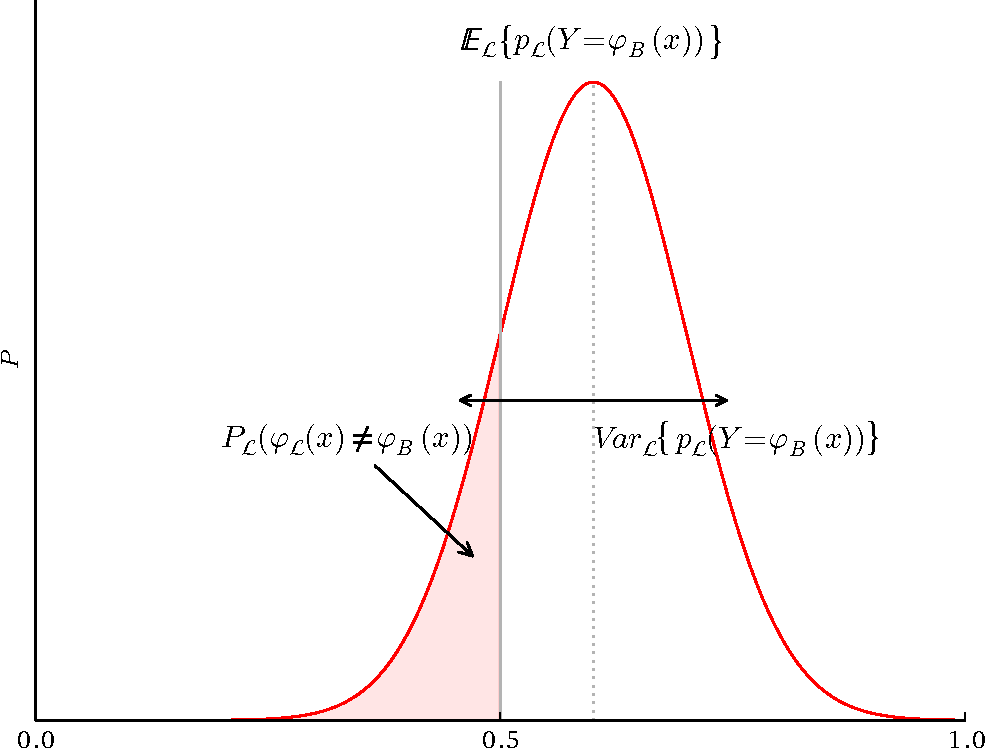
\includegraphics[width=0.9\textwidth]{figures/ch4_estimate_distribution.pdf}
    \caption{Probability distribution of the estimate $\widehat{p}_{\cal L}(Y=\varphi_B(\mathbf{x}))$.}
    \label{fig:estimate-distribution}
\end{figure}

If we now further assume\footnote{For single decision trees, the normal
assumption is certainly not satisfied in all cases, but the qualitative
conclusions are still generally valid. When the computations of the estimates
involve some averaging process, e.g., as further developed in the case of
ensemble of randomized trees, this approximation is however fairly reasonable.}
that the estimate $\widehat{p}_{\cal L}(Y=\varphi_B(\mathbf{x}))$ is normally distributed,
then probability~\ref{eqn:4:prob-diff-from-bayes} can be computed explicitly
from its mean and variance:
\begin{equation}
P_{\cal L}(\widehat{p}_{\cal L}(Y=\varphi_B(\mathbf{x})) < 0.5) = \Phi(\frac{0.5 - \mathbb{E}_{\cal L}\{ \widehat{p}_{\cal L}(Y=\varphi_B(\mathbf{x})) \}}{\sqrt{\mathbb{V}_{\cal L}\{ \widehat{p}_{\cal L}(Y=\varphi_B(\mathbf{x})) \}}})
\end{equation}
where $\Phi(x)=\frac{1}{\sqrt{2\pi}} \int_{-\infty}^x \exp(-\frac{t^2}{2}) dt$
is the cumulative distribution function of the standard normal distribution.
In summary, the expected generalization error additively
decomposes as formulated in Theorem~\ref{thm:bias-variance:classification}.

\begin{theorem}\label{thm:bias-variance:classification}
For the zero-one loss and binary classification, the expected
generalization error $\mathbb{E}_{\cal L} \{ Err(\varphi_{\cal L}(\mathbf{x}))
\}$ at $X=\mathbf{x}$ decomposes as follows:

\begin{align}
\mathbb{E}_{\cal L} \{ Err(\varphi_{\cal L}(\mathbf{x})) \} &= P(\varphi_B(\mathbf{x})\neq Y) \\
                                                            &+ \Phi(\frac{0.5 - \mathbb{E}_{\cal L}\{ \widehat{p}_{\cal L}(Y=\varphi_B(\mathbf{x})) \}}{\sqrt{\mathbb{V}_{\cal L}\{ \widehat{p}_{\cal L}(Y=\varphi_B(\mathbf{x})) \}}}) (2 P(\varphi_B(\mathbf{x}) = Y) - 1) \nonumber
\end{align}
\end{theorem}

As a result, Theorem~\ref{thm:bias-variance:classification} establishes a
direct connection between the regression variance of the estimates and the
classification error of the resulting model. In practice, this decomposition
has important consequences:
\begin{itemize}
\item When the expected probability estimate $\mathbb{E}_{\cal L}\{ \widehat{p}_{\cal L}(Y=\varphi_B(\mathbf{x}) \}$
      for the true majority class is greater than $0.5$, a reduction of
      variance of the estimate results in a decrease of the total misclassification
      error. If $\mathbb{V}_{\cal L}\{ \widehat{p}_{\cal L}(Y=\varphi_B(\mathbf{x})) \} \to 0$,
      then $\Phi \to 0$ and the expected generalization error tends to the error of the Bayes model.
      In particular, the generalization error can be driven to its minimum
      value whatever the regression bias of the estimate (at least as long as $\mathbb{E}_{\cal L}\{ \widehat{p}_{\cal L}(Y=\varphi_B(\mathbf{x}) \} > 0.5$).
\item Conversely, when $\mathbb{E}_{\cal L}\{ \widehat{p}_{\cal L}(Y=\varphi_B(\mathbf{x}) \} < 0.5$,
      a decrease of variance might actually increase the total misclassification error.
      If $\mathbb{V}_{\cal L}\{ \widehat{p}_{\cal L}(Y=\varphi_B(\mathbf{x})) \} \to 0$,
      then $\Phi \to 1$ and the error is maximal.
\end{itemize}


\section{Ensemble methods based on randomization}
\label{sec:4:ensemble}

Both theorems~\ref{thm:bias-variance} and \ref{thm:bias-variance:classification}
reveal the role of variance in the expected generalization error of a model. In
light of these results, a sensible approach for reducing generalization error
would therefore consist in driving down the prediction variance, provided the
respective bias can be kept the same or not be increased too much.

As it happens, \textit{ensemble methods} constitute a beautifully simple way to
do just that. Specifically, the core principle of ensemble methods based on randomization is to
introduce random perturbations into the learning procedure in order to produce
several different models from a single learning set ${\cal L}$ and then to
combine the predictions of those models to form the prediction of the ensemble.
How predictions are combined and why does it help is formally studied in the
next sections.


\subsection{Randomized models}

Given a learning set ${\cal L}$, a learning algorithm ${\cal A}$
deterministically produces a model ${\cal A}(\theta, {\cal L})$, denoted
$\varphi_{{\cal L},\theta}$\label{ntn:varphi-Ltheta}, where $\theta$ are
hyper-parameters controlling the execution of ${\cal A}$. Let us assume that $\theta$
includes a random seed parameter for mimicking some stochastic behavior in
${\cal A}$, hence producing (pseudo-)randomized models that are more or less
different from one random seed to another. (We defer the discussion on specific
random perturbations in the case of decision trees to Section~\ref{sec:4:random-forests}.)

In this context, the bias-variance decomposition can be extended to account for
everything that is random, hence considering both ${\cal L}$ and $\theta$ as
random variables\footnote{From now on, and without loss of generality, we
assume that the random variable $\theta$ only controls the randomness of the
learning algorithm.}.
Accordingly, theorems~\ref{thm:bias-variance} and \ref{thm:bias-variance:classification}
naturally extend to the expected generalization error
$\mathbb{E}_{{\cal L},\theta} \{ Err(\varphi_{{\cal L},\theta}(\mathbf{x})) \}$
of the randomized model $\varphi_{{\cal L},\theta}$ by replacing expectations
$\mathbb{E}_{\cal L} \{ . \}$ and variances $\mathbb{V}_{\cal L} \{ . \}$ with
their respective counterparts $\mathbb{E}_{{\cal L},\theta} \{ . \}$ and
$\mathbb{V}_{{\cal L},\theta} \{ . \}$ computed over the joint distribution of
${\cal L}$ and $\theta$. In regression, the bias-variance decomposition
of the squared error loss thus becomes:
\begin{equation}
\mathbb{E}_{{\cal L},\theta} \{ Err(\varphi_{{\cal L},\theta}(\mathbf{x})) \} = \text{noise}(\mathbf{x}) + \text{bias}^2(\mathbf{x}) + \text{var}(\mathbf{x}),
\end{equation}
where
\begin{align}
\text{noise}(\mathbf{x}) &= Err(\varphi_B(\mathbf{x})), \\
\text{bias}^2(\mathbf{x}) &= (\varphi_B(\mathbf{x}) - \mathbb{E}_{{\cal L},\theta} \{ \varphi_{{\cal L},\theta}(\mathbf{x}) \} )^2, \\
\text{var}(\mathbf{x}) &= \mathbb{E}_{{\cal L},\theta} \{ (\mathbb{E}_{{\cal L},\theta} \{ \varphi_{{\cal L},\theta}(\mathbf{x}) \} - \varphi_{{\cal L},\theta}(\mathbf{x}))^2 \}.
\end{align}

In this form, variance now accounts for both the prediction variability due to
the randomness of the learning set ${\cal L}$ and the variability due to the
randomness of the learning algorithm itself. As such, the variance of a
randomized algorithm is typically larger than the variance of its
deterministic counterpart. Depending on the strength of randomization, bias
also usually increases, but often to a smaller extent than variance.

While randomizing an algorithm might seem counter-intuitive, since it
increases both variance and bias, we will show in Section~\ref{sec:4:bias-variance:ensemble}
that combining several such randomized models might actually
achieve better performance than a single non-randomized model.


\subsection{Combining randomized models}

Let us assume a set of $M$\label{ntn:M} randomized models $\{\varphi_{{\cal L}, \theta_m} |
m = 1, \dots, M \}$, all learned on the same data ${\cal L}$ but each built
from an independent random seed $\theta_m$\label{ntn:theta-seed}\label{ntn:theta-seed-m}. Ensemble methods work by combining
the predictions of these models into a new \textit{ensemble} model, denoted
$\psi_{{\cal L},\theta_1,\dots,\theta_M}$\label{ntn:psi}, such that the expected
generalization error of the ensemble is (hopefully) smaller than the expected
generalization error of the individual randomized models.

In regression, for the squared error loss, the most common way to combine the
randomized models into an ensemble is to average their predictions to form the
final prediction:
\begin{equation}\label{eqn:4:averaging}
\psi_{{\cal L},\theta_1,\dots,\theta_M}(\mathbf{x}) = \frac{1}{M} \sum_{m=1}^M \varphi_{{\cal L},\theta_m}(\mathbf{x})
\end{equation}
The rationale is that the average prediction is the prediction that minimizes the average
squared error with respect to the individual predictions of the models. In that sense, the average prediction is the closest prediction with respect to all individual predictions.

\begin{remark}{Ambiguity decomposition}
For prediction averaging, as defined in Equation~\ref{eqn:4:averaging},
the \textit{ambiguity decomposition}~\citep{krogh:1995}
guarantees the generalization error of the ensemble to be lower
than the average generalization error of its constituents. Formally,
the ambiguity decomposition states that
\begin{equation}
Err(\psi_{{\cal L},\theta_1,\dots,\theta_M}) = \overline{E} - \overline{A}
\end{equation}
where
\begin{align}
\overline{E} &= \frac{1}{M} \sum_{m=1}^M Err(\varphi_{{\cal L},\theta_m}), \\
\overline{A} &= \mathbb{E}_{X} \{ \frac{1}{M} \sum_{m=1}^M (\varphi_{{\cal L},\theta_m}(X) - \psi_{{\cal L},\theta_1,\dots,\theta_M}(X))^2 \}.
\end{align}
The first term is the average generalization error of the individual models. The second term is the ensemble ambiguity and
corresponds to the variance of the individual predictions around the prediction of the ensemble. Since $\overline{A}$ is non-negative,
the generalization error of the ensemble is therefore smaller than the average generalization
error of its constituents.
\end{remark}

In classification, for the zero-one loss, predictions are usually aggregated by considering the
models in the ensemble as a committee  and then resorting to \textit{majority voting} to
form the final prediction:
\begin{equation}\label{eqn:4:majority-vote}
\psi_{{\cal L},\theta_1,\dots,\theta_M}(\mathbf{x}) = \argmax_{c \in {\cal Y}}  \sum_{m=1}^M 1(\varphi_{{\cal L},\theta_m}(\mathbf{x})=c)
\end{equation}
Similarly, the rationale is that the majority prediction is the prediction that minimizes
the average zero-one error with respect to the individual predictions.
Alternatively, when individual models provide class probability estimates $\widehat{p}_{{\cal L},\theta m}(Y=c|X=\mathbf{x})$,
\textit{soft voting}~\citep{zhou:2012}
consists in averaging the class probability estimates
and then predict the class which is the most likely:
\begin{equation}\label{eqn:4:avg-estimate}
\psi_{{\cal L},\theta_1,\dots,\theta_M}(\mathbf{x}) = \argmax_{c \in {\cal Y}} \frac{1}{M} \sum_{m=1}^M \widehat{p}_{{\cal L},\theta m}(Y=c|X=\mathbf{x})
\end{equation}
As empirically investigated by \citet{breiman:1996b}, both approaches yield
results that are nearly identical\footnote{In the case of ensembles of fully developed decision trees that perfectly classify all samples from ${\cal L}$, majority voting and soft voting are exactly equivalent.}. From a practical point of view however,
Equation~\ref{eqn:4:avg-estimate} has the advantage of providing smoother class
probability estimates for the ensemble, which may prove to be useful in
critical applications, e.g., when (estimates of) the certainty about
predictions is as important as the predictions themselves. Additionally,
combining predictions in this way makes it easy to study the expected
generalization error of the ensemble -- it suffices to plug the averaged
estimates into Theorem~\ref{thm:bias-variance:classification}. For these
reasons, and for the rest of this work, predictions in classification are now
assumed to be combined with soft voting (see Equation~\ref{eqn:4:avg-estimate}) unless
mentioned otherwise.

\begin{remark}{Condorcet's jury theorem}
Majority voting, as defined in Equation~\ref{eqn:4:majority-vote},
finds its origins in the \textit{Condorcet's jury theorem}
from the field of political science. Let consider a group of $M$ voters that
wishes to reach a decision by majority vote. The theorem states that if each
voter has an independent  probability $p > \tfrac{1}{2}$ of voting for the
correct decision, then adding more voters increases the probability of
the majority decision to be correct. When $M \to \infty$, the probability that the decision
taken by the group is correct approaches $1$. Conversely, if $p < \tfrac{1}{2}$, then
each voter is more likely to vote incorrectly and increasing $M$ makes things
worse.
\end{remark}

\subsection{Bias-variance decomposition of an ensemble}
\label{sec:4:bias-variance:ensemble}

Let us now study the bias-variance decomposition of the expected generalization
error of an ensemble $\psi_{{\cal L},\theta_1,\dots,\theta_M}$, first in the
case in case of regression and then for classification.

To simplify notations in the analysis below, let us denote the mean prediction at
$X=\mathbf{x}$ of a single randomized model $\varphi_{{\cal L},\theta_m}$ and its
respective prediction variance as:
\begin{align}
\mu_{{\cal L},\theta_m}(\mathbf{x}) &= \mathbb{E}_{{\cal L},\theta_m} \{ \varphi_{{\cal L},\theta_m}(\mathbf{x}) \} \label{eqn:4:mu} \\
\sigma^2_{{\cal L},\theta_m}(\mathbf{x}) &= \mathbb{V}_{{\cal L},\theta_m} \{ \varphi_{{\cal L},\theta_m}(\mathbf{x}) \label{eqn:4:sigma} \}
\end{align}

\subsubsection{Regression}

From Theorem~\ref{thm:bias-variance}, the expected generalization error of an
ensemble $\psi_{{\cal L},\theta_1,\dots,\theta_M}$ made of $M$ randomized
models decomposes into a sum of $\text{noise}(\mathbf{x})$,
$\text{bias}^2(\mathbf{x})$ and $\text{var}(\mathbf{x})$ terms.

The noise term only depends on the intrinsic randomness of $Y$. Its value
stays therefore the same, no matter the learning algorithm:
\begin{equation}
\text{noise}(\mathbf{x}) = \mathbb{E}_{Y|X=\mathbf{x}} \{ (Y - \varphi_B(\mathbf{x}))^2 \}
\end{equation}

The (squared) bias term is the (squared) difference between the prediction of the Bayes model
and the average prediction of the model. For an ensemble, the average prediction
is in fact the same as the average prediction of the corresponding randomized individual model. Indeed,
\begin{align}
\mathbb{E}_{{\cal L},\theta_1,\dots,\theta_M} \{ \psi_{{\cal L},\theta_1,\dots,\theta_M}(\mathbf{x}) \} &= \mathbb{E}_{{\cal L},\theta_1,\dots,\theta_M} \{ \frac{1}{M} \sum_{m=1}^M \varphi_{{\cal L},\theta_m}(\mathbf{x}) \} \nonumber \\
&= \frac{1}{M} \sum_{m=1}^M \mathbb{E}_{{\cal L},\theta_m} \{ \varphi_{{\cal L},\theta_m}(\mathbf{x}) \} \nonumber \\
&= \mu_{{\cal L},\theta}(\mathbf{x})
\end{align}
since random variables $\theta_m$ are independent and all follow the
same distribution. As a result,
\begin{equation}
\text{bias}^2(\mathbf{x}) = (\varphi_B(\mathbf{x}) - \mu_{{\cal L},\theta}(\mathbf{x}))^2,
\end{equation}
which indicates that the bias of an ensemble of randomized models is the same
as the bias of any of the randomized models. Put otherwise, combining
randomized models has no effect on the bias.

On variance on the other hand, ensemble methods show all their raison d'etre,
virtually reducing the variability of predictions to almost nothing and thereby
improving the accuracy of the ensemble. Before considering the variance of
$\psi_{{\cal L},\theta_1,\dots,\theta_M}(\mathbf{x})$ however, let us first
derive the correlation coefficient $\rho(\mathbf{x})$ between the predictions
of two randomized models built on the same learning set, but grown from two
independent random seeds $\theta^\prime$ and $\theta^{\prime\prime}$. From the definition of the Pearson's correlation
coefficient, it comes:
\begin{align}
\rho(\mathbf{x}) &= \frac{\mathbb{E}_{{\cal L},\theta^\prime,\theta^{\prime\prime}} \{ (\varphi_{{\cal L}, \theta^\prime}(\mathbf{x}) - \mu_{{\cal L},\theta^\prime}(\mathbf{x})) (\varphi_{{\cal L}, \theta^{\prime\prime}}(\mathbf{x}) - \mu_{{\cal L},\theta^{\prime\prime}}(\mathbf{x})) \}}{\sigma_{{\cal L},\theta^\prime}(\mathbf{x}) \sigma_{{\cal L},\theta^{\prime\prime}}(\mathbf{x})} \nonumber \\
&= \frac{\mathbb{E}_{{\cal L},\theta^\prime,\theta^{\prime\prime}} \{ \varphi_{{\cal L},\theta^\prime}(\mathbf{x}) \varphi_{{\cal L},\theta^{\prime\prime}}(\mathbf{x}) - \varphi_{{\cal L},\theta^\prime}(\mathbf{x}) \mu_{{\cal L},\theta^{\prime\prime}}(\mathbf{x}) - \varphi_{{\cal L},\theta^{\prime\prime}}(\mathbf{x}) \mu_{{\cal L},\theta^\prime}(\mathbf{x}) + \mu_{{\cal L},\theta^\prime}(\mathbf{x}) \mu_{{\cal L},\theta^{\prime\prime}}(\mathbf{x}) \}}{\sigma^2_{{\cal L},\theta}(\mathbf{x})} \nonumber \\
&= \frac{\mathbb{E}_{{\cal L},\theta^\prime,\theta^{\prime\prime}} \{ \varphi_{{\cal L},\theta^\prime}(\mathbf{x}) \varphi_{{\cal L},\theta^{\prime\prime}}(\mathbf{x}) \} - \mu^2_{{\cal L},\theta}(\mathbf{x})}{\sigma^2_{{\cal L},\theta}(\mathbf{x})} \label{eqn:4:correlation}
\end{align}
by linearity of the expectation and exploiting the fact that random variables
$\theta^\prime$ and $\theta^{\prime\prime}$ follow the same distribution.
Intuitively, $\rho(\mathbf{x})$ represents the strength of the random
perturbations introduced in the learning algorithm. When it is close to $1$,
predictions of two randomized models are highly correlated, suggesting that
randomization has no sensible effect on the predictions. By contrast, when it
is close to $0$, predictions of the randomized models are decorrelated, hence
indicating that randomization has a strong effect on the predictions. At the
limit, when $\rho(\mathbf{x})=0$, predictions of two models built on the same
learning set ${\cal L}$ are independent, which happens when they are perfectly
random. As proved later with Equation~\ref{eqn:4:correlation-bis}, let us
finally also remark that the correlation term $\rho(\mathbf{x})$
is non-negative, which confirms that randomization has a decorrelation effect
only.

From Equation~\ref{eqn:4:correlation}, the variance of $\psi_{{\cal
L},\theta_1,\dots,\theta_M}(\mathbf{x})$ can now be derived as follows:
\begin{align}
\text{var}(\mathbf{x}) &= \mathbb{V}_{{\cal L},\theta_1,\dots,\theta_M} \{ \frac{1}{M} \sum_{m=1}^M \varphi_{{\cal L},\theta_m}(\mathbf{x})  \} \nonumber \\
&= \frac{1}{M^2} \Bigg[ \mathbb{E}_{{\cal L},\theta_1,\dots,\theta_M} \{ (\sum_{m=1}^M \varphi_{{\cal L},\theta_m}(\mathbf{x}))^2 \} - \mathbb{E}_{{\cal L},\theta_1,\dots,\theta_M} \{ \sum_{m=1}^M \varphi_{{\cal L},\theta_m}(\mathbf{x}) \}^2 \Bigg] \nonumber
\end{align}
by exploiting the facts that $\mathbb{V}\{a X\} = a^2 \mathbb{V}\{ X \}$,
$\mathbb{V}\{ X \} = \mathbb{E}\{X^2\} - \mathbb{E}\{ X \}^2$ and the linearity
of expectation. By rewriting the square of the sum of the $\varphi_{{\cal L},\theta_m}(\mathbf{x})$ terms as a sum over all pairwise products $\varphi_{{\cal L},\theta_i}(\mathbf{x}) \varphi_{{\cal L},\theta_j}(\mathbf{x})$, the variance can further be rewritten as:
\begin{align}
&= \frac{1}{M^2} \Bigg[ \mathbb{E}_{{\cal L},\theta_1,\dots,\theta_M} \{ \sum_{i,j} \varphi_{{\cal L},\theta_i}(\mathbf{x}) \varphi_{{\cal L},\theta_j}(\mathbf{x}) \} - (M \mu_{{\cal L},\theta}(\mathbf{x}))^2 \Bigg] \nonumber \\
&= \frac{1}{M^2} \Bigg[ \sum_{i,j} \mathbb{E}_{{\cal L},\theta_i,\theta_j} \{  \varphi_{{\cal L},\theta_i}(\mathbf{x}) \varphi_{{\cal L},\theta_j}(\mathbf{x}) \} - M^2 \mu^2_{{\cal L},\theta}(\mathbf{x}) \Bigg] \nonumber \\
&= \frac{1}{M^2} \Bigg[ M \mathbb{E}_{{\cal L},\theta} \{ \varphi_{{\cal L},\theta}(\mathbf{x})^2 \} \nonumber \\
&\quad \hookrightarrow + (M^2-M) \mathbb{E}_{{\cal L},\theta^\prime,\theta^{\prime\prime}} \{  \varphi_{{\cal L},\theta^\prime}(\mathbf{x}) \varphi_{{\cal L},\theta^{\prime\prime}}(\mathbf{x}) \}  - M^2 \mu^2_{{\cal L},\theta}(\mathbf{x}) \Bigg] \nonumber \\
&= \frac{1}{M^2} \Bigg[ M (\sigma^2_{{\cal L},\theta}(\mathbf{x}) + \mu^2_{{\cal L},\theta}(\mathbf{x})) \nonumber \\
&\quad \hookrightarrow + (M^2-M)(\rho(\mathbf{x}) \sigma^2_{{\cal L},\theta}(\mathbf{x}) + \mu^2_{{\cal L},\theta}(\mathbf{x})) - M^2 \mu^2_{{\cal L},\theta}(\mathbf{x}) \Bigg] \nonumber \\
&= \frac{\sigma^2_{{\cal L},\theta}(\mathbf{x})}{M} + \rho(\mathbf{x})\sigma^2_{{\cal L},\theta}(\mathbf{x}) - \rho(\mathbf{x}) \frac{\sigma^2_{{\cal L},\theta}(\mathbf{x})}{M} \nonumber \\
&= \rho(\mathbf{x}) \sigma^2_{{\cal L},\theta}(\mathbf{x}) + \frac{1 - \rho(\mathbf{x})}{M} \sigma^2_{{\cal L},\theta}(\mathbf{x}) \label{eqn:4:variance-hastie}
\end{align}
As the size of the ensemble gets arbitrarily large, i.e., as $M \to \infty$,
the variance of the ensemble reduces to $\rho(\mathbf{x})
\sigma^2_{{\cal L},\theta}(\mathbf{x})$. Under the assumption that randomization has some
effect on the predictions of randomized models, i.e., assuming
$\rho(\mathbf{x}) < 1$, the variance of an ensemble is therefore strictly
smaller than the variance of an individual model. As a result, the expected
generalization error of an ensemble is strictly smaller than the expected error
of a randomized model. As such, improvements in predictions are
solely the result of variance reduction, since both $\text{noise}(\mathbf{x})$
and $\text{bias}^2(\mathbf{x})$ remain unchanged. Additionally, when random
effects are strong, i.e., when $\rho(\mathbf{x}) \to 0$, variance reduces to
$\smash{\tfrac{\sigma^2_{{\cal L},\theta}(\mathbf{x})}{M}}$, which can further be driven to $0$ by
increasing the size of the ensemble. On the other hand, when random effects are weak,
i.e., when $\rho(\mathbf{x}) \to 1$, then variance reduces to $\sigma^2_{{\cal
L},\theta}(\mathbf{x})$ and building an ensemble brings no benefit. Put otherwise, the stronger the random effects, the larger
the reduction of variance due to ensembling, and vice-versa.

In summary, the expected generalization error of an ensemble additively
decomposes as stated in Theorem~\ref{thm:bias-variance:ensemble}.
\begin{theorem}\label{thm:bias-variance:ensemble}
For the squared error loss, the bias-variance decomposition of the expected
generalization error $\mathbb{E}_{\cal L} \{ Err( \psi_{{\cal L},\theta_1,\dots,\theta_M}(\mathbf{x}))
\}$ at $X=\mathbf{x}$ of an ensemble of $M$ randomized models $\varphi_{{\cal L},\theta_m}$ is
\begin{equation}
\mathbb{E}_{\cal L} \{ Err(\psi_{{\cal L},\theta_1,\dots,\theta_M}(\mathbf{x})) \} = \text{noise}(\mathbf{x}) + \text{bias}^2(\mathbf{x}) + \text{var}(\mathbf{x}),
\end{equation}
where
\begin{align*}
\text{noise}(\mathbf{x}) &= Err(\varphi_B(\mathbf{x})), \\
\text{bias}^2(\mathbf{x}) &= (\varphi_B(\mathbf{x}) - \mathbb{E}_{{\cal L},\theta} \{ \varphi_{{\cal L},\theta}(\mathbf{x}) \} )^2, \\
\text{var}(\mathbf{x}) &= \rho(\mathbf{x}) \sigma^2_{{\cal L},\theta}(\mathbf{x}) + \frac{1 - \rho(\mathbf{x})}{M} \sigma^2_{{\cal L},\theta}(\mathbf{x}).
\end{align*}
\end{theorem}

In light of Theorem~\ref{thm:bias-variance:ensemble}, the core principle of
ensemble methods is thus to introduce random perturbations in order to
decorrelate as much as possible the predictions of the individual models,
thereby maximizing variance reduction. However, random perturbations need to be
carefully chosen so as to increase bias as little as possible.  The crux of the
problem is to find the right trade-off between randomness and bias.

\begin{remark}{Alternative variance decomposition}
\citet{geurts:2002} (Chapter 4, Equation~4.31) alternatively decomposes the ensemble variance as
\begin{equation}\label{eqn:4:variance-geurts}
\text{var}(\mathbf{x}) = \mathbb{V}_{\cal L} \{ \mathbb{E}_{\theta|{\cal L}} \{ \varphi_{{\cal L},\theta}(\mathbf{x}) \} \} + \frac{1}{M} \mathbb{E}_{\cal L} \{ \mathbb{V}_{\theta|{\cal L}} \{ \varphi_{{\cal L},\theta}(\mathbf{x}) \} \}.
\end{equation}
The first term of this decomposition is the variance due to the randomness
of the learning set ${\cal L}$, averaged over the random perturbations due to $\theta$. It
measures the dependence of the model on the learning set, independently of
$\theta$. The second term is the expectation over all learning sets of
the variance with respect to $\theta$. It measures the strength of the
random effects. As the decomposition shows, only this last part of the variance
can be reduced as a result of averaging, which is consistent with our previous
conclusions.  The stronger the random effects, the larger the variance with
respect to $\theta$, and hence the larger of reduction of variance due
to ensembling.

\begin{proposition}Decompositions \ref{eqn:4:variance-hastie} and \ref{eqn:4:variance-geurts} of the prediction variance for an ensemble are equivalent.
\end{proposition}

\begin{proof}
From Equations~\ref{eqn:4:variance-hastie} and \ref{eqn:4:variance-geurts}, equivalence holds if Equation~\ref{eqn:4:correlation}
is equivalent to
\begin{equation}\label{eqn:4:correlation-bis}
\rho(\mathbf{x}) = \frac{\mathbb{V}_{\cal L} \{ \mathbb{E}_{\theta|{\cal L}} \{ \varphi_{{\cal L},\theta}(\mathbf{x}) \} \}}{\mathbb{V}_{\cal L} \{ \mathbb{E}_{\theta|{\cal L}} \{ \varphi_{{\cal L},\theta}(\mathbf{x}) \} \} + \mathbb{E}_{\cal L} \{ \mathbb{V}_{\theta|{\cal L}} \{ \varphi_{{\cal L},\theta}(\mathbf{x}) \} \}}.
\end{equation}
From the law of total variance, the denominator of Equation~\ref{eqn:4:correlation} expands
to the denominator of Equation~\ref{eqn:4:correlation-bis}:
\begin{equation}
\sigma^2_{{\cal L},\theta}(\mathbf{x}) = \mathbb{V}_{\cal L} \{ \mathbb{E}_{\theta|{\cal L}} \{ \varphi_{{\cal L},\theta}(\mathbf{x}) \} \} + \mathbb{E}_{\cal L} \{ \mathbb{V}_{\theta|{\cal L}} \{ \varphi_{{\cal L},\theta}(\mathbf{x}) \} \}
\end{equation}
Similarly, the numerator of Equation~\ref{eqn:4:correlation-bis} can be reexpressed
as the numerator of Equation~\ref{eqn:4:correlation}, thereby proving the equivalence:
\begin{align}
& \mathbb{V}_{\cal L} \{ \mathbb{E}_{\theta|{\cal L}} \{ \varphi_{{\cal L},\theta}(\mathbf{x}) \} \} \nonumber \\
&= \mathbb{E}_{\cal L} \{ (\mathbb{E}_{\theta|{\cal L}} \{ \varphi_{{\cal L},\theta}(\mathbf{x}) \} - \mathbb{E}_{\cal L} \{ \mathbb{E}_{\theta|{\cal L}} \{ \varphi_{{\cal L},\theta}(\mathbf{x})\} \})^2 \} \nonumber \\
&= \mathbb{E}_{\cal L} \{ (\mathbb{E}_{\theta|{\cal L}} \{ \varphi_{{\cal L},\theta}(\mathbf{x}) \} - \mu_{{\cal L},\theta}(\mathbf{x}))^2 \} \nonumber \\
&= \mathbb{E}_{\cal L} \{ \mathbb{E}_{\theta|{\cal L}} \{ \varphi_{{\cal L},\theta}(\mathbf{x}) \}^2 \} - \mu^2_{{\cal L},\theta}(\mathbf{x}) \nonumber \\
&= \mathbb{E}_{\cal L} \{ \mathbb{E}_{\theta^\prime|{\cal L}} \{ \varphi_{{\cal L},\theta^\prime}(\mathbf{x}) \} \mathbb{E}_{\theta^{\prime\prime}|{\cal L}} \{ \varphi_{{\cal L},\theta^{\prime\prime}}(\mathbf{x}) \} \} - \mu^2_{{\cal L},\theta}(\mathbf{x}) \nonumber \\
&= \mathbb{E}_{{\cal L},\theta^\prime,\theta^{\prime\prime}} \{ \varphi_{{\cal L},\theta^\prime}(\mathbf{x}) \varphi_{{\cal L},\theta^{\prime\prime}}(\mathbf{x}) \} - \mu^2_{{\cal L},\theta}(\mathbf{x}).
\end{align}
\end{proof}

In this form, $\rho(\mathbf{x})$ is interpreted as the ratio between the variance
due to the learning set  and the total variance, accounting for
random effects due to both the learning set and the random perturbations.
It is close to $1$ when variance is mostly due to the learning set, hence
yielding correlated predictions. Conversely, it is close to $0$ when variance
is mostly due to the random perturbations induced by $\theta$, hence decorrelating
the predictions.
\end{remark}

\subsubsection{Classification}

The decomposition of the expected generalization error of an ensemble in
classification directly follows from theorems~\ref{thm:bias-variance:classification} and
\ref{thm:bias-variance:ensemble}.
Building an ensemble always reduces the variance of the class probability estimate
$\mathbb{E}_{{\cal L},\theta}\{ \widehat{p}_{{\cal
L},\theta}(Y=\varphi_B(\mathbf{x}) \}$ (as shown in Equation~\ref{eqn:4:variance-hastie}), which results in a decrease of the misclassification error
if the expected estimate remains strictly greater than $0.5$ in a
randomized model.

\begin{remark}{Shortcomings addressed by ensembles}
In complement with the formal bias-variance analysis carried out in the previous
section, \citet{dietterich:2000b} identifies three fundamental reasons
intuitively explaining why ensembles often work better than single models.

The first reason is statistical. When the learning set is too small, a learning
algorithm can typically find several models in the hypothesis space ${\cal H}$
that all give the same performance on the training data. Provided their predictions
are uncorrelated, averaging several models reduces the risk of choosing the wrong hypothesis.

The second reason is computational. Many learning algorithms rely on some
greedy assumption or local search that may get stuck in local optima. As such, an ensemble
made of individual models built from many different starting points may provide
a better approximation of the true unknown function that any of the single
models.

Finally, the third reason is representational. In most cases, for a learning set of finite size, the true
function cannot be represented by any of the candidate models in ${\cal H}$.
By combining several models in an ensemble, it may be possible to expand the space
of representable functions and to better model the true function.
\end{remark}


\section{Random Forests}
\label{sec:4:random-forests}

Random forests\footnote{The term
\textit{random forests}, without capitals, is used to denote any ensemble of decision
trees. Specific variants are referred to using their original designation,
denoted with capitals. In particular, the ensemble method due to
\citet{breiman:2001} is denoted as \textit{Random Forests}, with capitals.}
form a family of methods that consist in building an ensemble (or
\textit{forest}) of decision trees grown from a randomized variant of the tree
induction algorithm (as described in Chapter~\ref{ch:cart}). Decision trees are
indeed ideal candidates for ensemble methods since they usually have low bias
and high variance, making them very likely to benefit from the averaging
process. As we will review in this section, random forests methods mostly
differ from each other in the way they introduce random perturbations into the
induction procedure. As highlighted in the previous section, the difficulty is
to inject randomness while minimizing $\rho(\mathbf{x})$ and
simultaneously maintaining a low bias in the randomized decision trees.

\subsection{Randomized induction algorithms}

\begin{description}

\item \citet{kwok:1990}: \hfill \\
    Historically, the earliest mention of ensemble of decision trees is due to
    \citet{kwok:1990}. In this work, the authors empirically observe that
    averaging multiple decision trees with different structure consistently
    produces better results than any of the constituents of the ensemble. This
    approach however was not based on randomization nor was fully automatic:
    decision trees were generated by first manually selecting at the top of the
    tree splits that were almost as good as the optimal splits, and then
    expanded using the classical ID3 induction procedure.

\item \citet{breiman:1996b}: \hfill \\
    In a now famous technical report, \citet{breiman:1996b} was one of the earliest to
    show, both theoretically and empirically, that aggregating multiple
    versions of an estimator into an ensemble can give substantial gains in
    accuracy. He notes and shows that the average model $\mathbb{E}_{\cal L}\{
    \varphi_{\cal L} \}$ has a lower expected generalization error than
    $\varphi_{\cal L}$. As such, \textit{Bagging}  consists in
    approximating $\mathbb{E}_{\cal L}\{ \varphi_{\cal L} \}$  by combining
    models built from \textit{bootstrap samples}~\citep{efron:1979} ${\cal
    L}^m$\label{ntn:L_m} (for $m=1,\dots,M$) of the learning set ${\cal L}$. The $\{ {\cal
    L}^m \}$ form replicates of ${\cal L}$, each consisting of $N$ cases $(\mathbf{x},y)$, drawn
    at random but \textit{with replacement} from ${\cal L}$.

    Note that even
    though $|{\cal L}|=|{\cal L}^m|=N$, $37\%$ of the couples $(\mathbf{x},y)$ from ${\cal L}$
    are on average missing in the bootstrap replicates. Indeed, after $N$ draws
    with replacement, the probability of never have been selected is
    \begin{equation}
    (1 - \frac{1}{N})^N \approx \frac{1}{e} \approx 0.368.
    \end{equation}
    When the learning algorithm is unstable (i.e., when small changes in the
    learning set can cause large changes in the learned models), Bagging
    generates individual models that are  different from one bootstrap sample
    to another, hence making them likely to benefit from the averaging process.
    In some cases however, when the learning set ${\cal L}$ is small,
    subsampling $67\%$ of the objects might lead to an increase of bias
    (e.g., because of a decrease in model complexity) which
    is too large to be compensated by a decrease of variance, hence resulting
    in overall poorer performance. Despite this defect, Bagging has proven to
    be an effective method in numerous applications, one of its strengths being
    that it can be used to combine any kind of models -- i.e., not only
    decision trees.

\item \citet{dietterich:1995}: \hfill \\
    Building upon \citep{kwok:1990}, \citet{dietterich:1995} propose
    to randomize the choice of the best split at a given node by selecting
    uniformly at random one of the $20$ best splits of node $t$. The authors empirically
    show in \citep{dietterich:1995,dietterich:2000} that randomizing in this
    way gives results that are slightly better than Bagging in low noise settings.
    Experiments show however that when noise is important, Bagging usually
    yield better results. From a bias-variance point of view, this method
    virtually does not change bias but increases variance due to randomization.

\item \citet{amit:1997}: \hfill \\
    In the context of handwritten character recognition, where the number $p$
    of input variables is typically very large, \citet{amit:1997} propose a
    randomized variant of the tree induction algorithm that consists in
    searching for the best split at each node over a random subsample of the
    variables.

    Denoting $K \leq p$\label{ntn:K-split} (also known as \texttt{mtry} or
    \texttt{max\_features}) the number of variables effectively considered at
    each node, this variant replaces Algorithm~\ref{algo:findsplit}
    with the following randomized alternative:
    \begin{algorithm}\label{algo:findsplit:random}
    Find the best split $s^*$ that partitions ${\cal L}_t$, among a random subset of $K \leq p$ input variables.
    \textnormal{
    \begin{algorithmic}[1]
    \Function{FindBestSplitRandom}{${\cal L}_t$, $K$}
        \State $\Delta = -\infty$
        \State Draw $K$ random indices $j_k$ from $1,\dots,p$
        \For{$k=1, \dots, K$}
            \State Find the best binary split $s^*_{j_k}$ defined on $X_{j_k}$
            \If{$\Delta i(s^*_{j_k}, t) > \Delta$}
                \State $\Delta = \Delta i(s^*_{j_k}, t)$
                \State $s^* = s^*_{j_k}$
            \EndIf
        \EndFor
        \State \Return $s^*$
    \EndFunction
    \end{algorithmic}
    }
    \end{algorithm}
    When the output $Y$ can be explained in several ways, this randomized
    algorithm generates trees that are each structurally different, yet
    individually good. As a result, bias usually increases only slightly, while
    the increased variance due to randomization can be cancelled out through averaging. The
    optimal trade-off between these quantities can otherwise be adjusted by
    tuning the value of $K$. As $K \to 1$, the larger the bias but the larger the
    variance of the individual models and hence the more effective the
    averaging process. Conversely, as $K \to p$, the smaller the bias but also the
    smaller the variance of the individual models and therefore the less
    beneficial the ensemble.

\item \citet{ho:1998}: \hfill \\
    Inspired from the principles of Bagging~\citep{breiman:1996b} and
    random subsets of variables~\citep{amit:1997}, \citet{ho:1998} proposes
    with the \textit{Random Subspace} (RS) method to build a \textit{decision
    forest} whose trees are grown on random subsets of the input variables
    -- drawn once, prior to the construction of each tree -- rather than on all $p$
    variables. As empirically evaluated at several
    occasions~\citep{ho:1998,panov:2007,louppe:2012}, the Random Subspace
    method is a powerful generic ensemble method that can achieve near state-of-the-art
    performance on many problems. Again, the optimal trade-off between the
    variance due to randomization  and the increase of bias can be controlled
    by tuning the size of the random subset.

\item \citet{breiman:2001}: \hfill \\
    In his seminal \textit{Random Forests} (RF) paper, \citet{breiman:2001} combines
    Bagging~\citep{breiman:1996b} with random variable selection at each
    node~\citep{amit:1997}. Injecting randomness simultaneously with both strategies  yields
    one the most effective off-the-shelf methods in machine learning, working
    surprisingly well for almost any kind of problems. The author empirically
    shows that Random Forests give results that are competitive with
    boosting \citep{freund:1995} and arcing algorithms \citep{breiman:1996},
    which both are designed to reduce bias while forests focus on variance
    reduction.

    While the original principles are due to several authors (as discussed
    above), Breiman is often cited as the father of forests of randomized trees. Parts of
    this recognition are certainly due to the pioneer theoretical analysis that
    has always complemented his empirical analysis of algorithms. In contrast
    with other authors, another reason might also be his efficient software
    implementation~\citep{breiman:2002} that was made freely available,
    allowing users outside of the machine learning community to quickly and
    easily apply Random Forests to their problems.

\item \citet{cutler:2001}: \hfill \\
    With \textit{Perfect Random Tree Ensembles} (PERT), \citet{cutler:2001}
    propose to grow a forest of perfectly fit decision trees in which both the
    (ordered) variable to split on and the discretization threshold are chosen
    at random. More specifically, given a node $t$, the split variable $X_j$ is
    drawn at random using Algorithm~\ref{algo:findsplit:random} with $K=1$
    while the cut-point $v$ is set midway between two randomly drawn samples using
    the following procedure (instead of Algorithm~\ref{algo:findsplit:x_j}):
    \begin{algorithm}\label{algo:findsplit:pert}
    Draw a random split on $X_j$ that partitions ${\cal L}_t$.
    \textnormal{
    \begin{algorithmic}[1]
    \Function{FindRandomSplit-PERT}{${\cal L}_t$, $X_j$}
        \State Draw $(\mathbf{x}_1,y_1), (\mathbf{x}_2,y_2) \in {\cal L}_t$ such that $y_1 \neq y_2$
        \State Draw $\alpha$ uniformly at random from $[0,1]$
        \State $v = \alpha x_{1,j} + (1 -\alpha) x_{2, j}$
        \State \Return $s^v_j$
    \EndFunction
    \end{algorithmic}
    }
    \end{algorithm}
    The induction of the tree proceeds using such random splits until
    all nodes become pure or until it is no longer possible to draw samples
    of different output values.

    From a practical point of view, PERT is an easily coded and a very
    efficient ensemble method since there is no impurity criterion to evaluate
    when splitting the nodes of a tree. Regarding accuracy, experimental
    comparisons in \citep{cutler:2001} show that PERT is often nearly as good as
    Random Forests \citep{breiman:2001}, while resulting however in random
    trees that are typically larger than  decision trees grown with
    less randomization. The simplicity of the method also allows for an amenable
    theoretical analysis of forests of randomized trees, as carried out in \citep{zhao:2000}.

\item \citet{geurts:2006}: \hfill \\
    As investigated in \citep{wehenkel:1997,geurts:2000},  the notoriously high
    variance of decision trees partly finds its origins from the high
    dependence of the splits with the random nature of the learning set. The
    authors empirically show that the variance of the optimal cut-point $v$ (in
    the case of ordered input variables) may indeed be very high, even for
    large sample sizes.  In particular, \citet{geurts:2002} shows that cut-point
    variance appears to be responsible for a significant part of the
    generalization error of decision trees. As a way to smoothen the decision
    boundary, \citet{geurts:2006} hence propose in \textit{Extremely Randomized
    Trees} (ETs) to combine random variable selection~\citep{amit:1997} with
    random discretization thresholds. As a drop-in replacement of Algorithm~\ref{algo:findsplit:x_j},
    the authors propose the following simplistic but effective
    procedure for drawing splits at random:
    \begin{algorithm}\label{algo:findsplit:et}
    Draw a random split on $X_j$ that partitions ${\cal L}_t$.
    \textnormal{
    \begin{algorithmic}[1]
    \Function{FindRandomSplit-ETs}{${\cal L}_t$, $X_j$}
        \State $\min_j = \min(\{ x_{i,j} | (\mathbf{x}_i,y_i) \in {\cal L}_t \})$
        \State $\max_j = \max(\{ x_{i,j} | (\mathbf{x}_i,y_i) \in {\cal L}_t \})$
        \State Draw $v$ uniformly at random from $[\min_j, \max_j[$
        \State \Return $s^v_j$
    \EndFunction
    \end{algorithmic}
    }
    \end{algorithm}
    With respect to decomposition~\ref{eqn:4:variance-geurts} of variance,
    extremely randomized trees can therefore be seen as a way to transfer
    cut-point variance from the variance term due to the learning
    set to the (reducible) variance term that is due to random effects.

    In the special case where $K=1$, Extremely Randomized Trees reduce to
    \textit{Totally Randomized Trees}, in which both a single variable $X_j$
    and a discretization threshold $v$ are drawn at random at each node. As a
    result, the structure of such trees can be learned in an unsupervised way,
    independently of the output variable $Y$. In this setting, Totally
    Randomized Trees are very close to Perfect Random Tree
    Ensembles~\citep{cutler:2001} since both draw $X_j$ and $v$ at random.
    These methods are however not strictly equivalent since they do not draw
    the random discretization thresholds $v$ with respect to the same
    probability distribution.

\item \citet{rodriguez:2006}: \hfill \\
    In a different direction, \citet{rodriguez:2006} propose in
    \textit{Rotation Forests} to generate randomized decision trees based on
    feature extraction. As in Bagging~\citep{breiman:1996b}, individual
    decision trees are built on bootstrap replicates ${\cal L}^m$ of the
    learning set ${\cal L}$. To further enhance diversity (i.e., to further
    decorrelate the predictions of the constituents of the ensemble), for each
    of the $M$ bootstrap replicates, input variables are randomly partitioned
    into $q$  subsets of $\tfrac{p}{q}$ variables, principal component analysis
    (PCA) is run separately on each subset, and a new set
    $\smash{\widetilde{{\cal L}^m}}$ of $p$ extracted input variables is
    constructed by pooling all principal components from the $q$ projections.
    In this way, bootstrap replicates ${\cal L}^m$ are each independently
    transformed linearly into a new input space using $q$  axis rotations. In
    this framework,  decision trees are particularly suited because they are
    sensitive to changes in the input space and still can be very accurate. As
    reported in \citep{rodriguez:2006,kuncheva:2007}, Rotation Forests
    favorably compare with other tree-based ensemble methods, yielding results
    that are often as good, sometimes better, than Random
    Forests~\citep{breiman:2001}. In terms of complexity however, the computational
    overhead due to the $q$ axis rotations should not be overlooked when
    resources are limited.

\end{description}

\subsection{Illustration}
\label{sec:4:illustration}

As a summary and illustrative example, let us consider a simulated toy
regression problem such that
\begin{equation}
Y = \sum_{j=1}^{5} X_j,
\end{equation}
where all input variables $X_1,\dots,X_{5}$ are independent
random Gaussian variables of zero mean and unit variance. To simulate
noise in the data, 5 additional random Gaussian input variables $X_{6},\dots,X_{10}$,
all independent from $Y$, are further appended to the learning set.

Let us compare for this problem the bias-variance decomposition of the expected
generalization error of a Random Forest~\citep{breiman:2001} (RF) and of
Extremely Randomized Trees~\citep{geurts:2006} (ETs). For both methods, the
error is estimated as derived from Theorem~\ref{thm:bias-variance:ensemble},
using $100$ randomly drawn learning sets ${\cal L}$ of $50$ samples, on which
ensembles of $10$ trees are built. Their generalization error is estimated on
an independent test set of $1000$ samples.

\begin{figure}
    \centering
    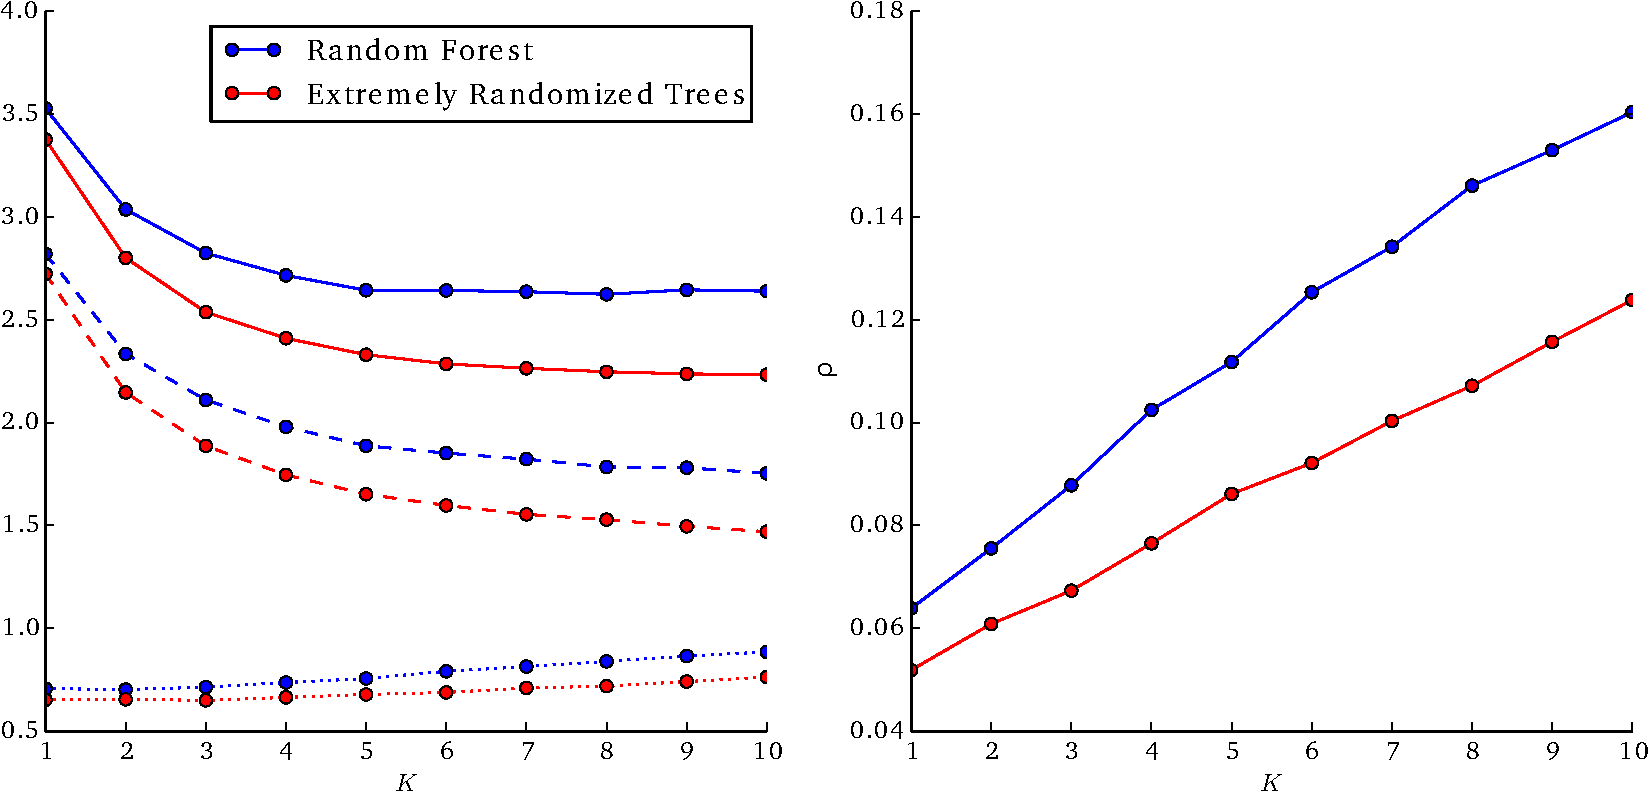
\includegraphics[width=\textwidth]{figures/ch4_correlation.pdf}
    \caption{(Left) Bias-variance decomposition of the generalization error
            with respect to the hyper-parameter $K$. The total error is shown by the plain
            lines. Bias and variance terms are respectively shown by the dashed and dotted
            lines.  (Right) Average correlation
            coefficient $\rho(\mathbf{x})$ over the predictions of two randomized trees
            grown from the same learning set but with different random seeds.}
    \label{fig:correlation}
\end{figure}
\begin{figure}
    \centering
    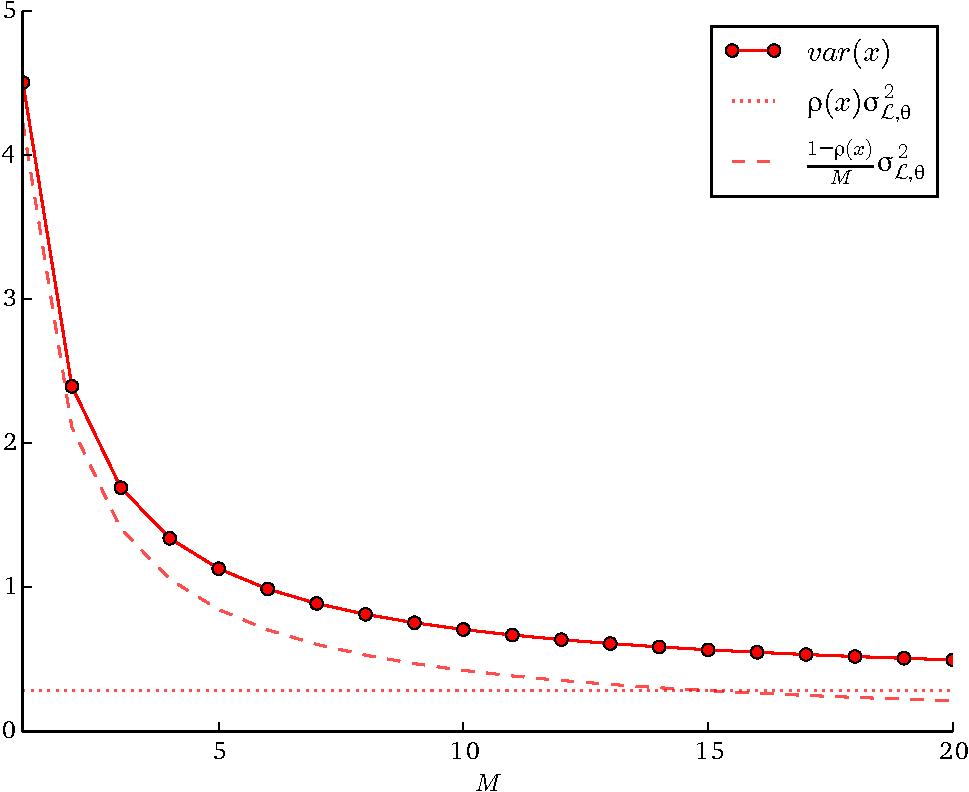
\includegraphics[width=0.9\textwidth]{figures/ch4_variance.pdf}
    \caption{Decomposition of the variance term $\text{var}(\mathbf{x})$ with respect to the number $M$ of trees in the ensemble.}
    \label{fig:variance}
\end{figure}

As the left plot in Figure~\ref{fig:correlation} shows,  the expected
generalization error additively decomposes into (squared) bias and variance
terms.  For small values of $K$, random effects are strong, leading to high
bias and low variance. By contrast, for larger values of $K$, random effects
are less important, reducing bias but increasing variance.   For both methods,
too small a value of $K$ appears however to lead to a too large increase of
bias, for which averaging is not able to compensate. For RF, the optimal
trade-off is at $K=8$, which indicates that bagging and random variable selection are
here complementary with regard to the level of randomness injected into the
trees. Indeed, using bagging only (at $K=10$) for randomizing the construction
of the trees yield results that are slightly worse than when both techniques
are combined. For ETs, the optimal trade-off is at $K=10$, suggesting that
random thresholds $v$ provide by themselves enough randomization on this
problem.

The right plot of Figure~\ref{fig:correlation} illustrates the (averaged)
correlation coefficient $\rho(\mathbf{x})$ between the predictions of two
randomized trees grown on the same learning set. As expected, the smaller $K$,
the stronger the random effects, therefore the less correlated the predictions
and the more variance can be reduced from averaging. The plot also confirms
that ETs are inherently less correlated than trees built
in RF, which is not surprising given the fact that the former
method randomizes the choice of the discretization threshold while the latter
does not. In cases where such a randomization does not induce too large an
increase of bias, as in this problem, ETs are therefore
expected to yield better results than RF.  (The choice of the
optimal randomization strategy is however highly dependent on the problem and
no general conclusion should be drawn from this toy regression problem.)

As confirmed by Figure~\ref{fig:variance} for RF, variance also additively decomposes  into
\begin{equation}
\text{var}(\mathbf{x}) = \rho(\mathbf{x}) \sigma^2_{{\cal L},\theta}(\mathbf{x}) + \tfrac{1 - \rho(\mathbf{x})}{M} \sigma^2_{{\cal L},\theta}(\mathbf{x}).
\end{equation}
The first term is the variance due to the learning set ${\cal L}$ and remains
constant as the number $M$ of trees increases. The second term is the variance
due to random effects and decreases as $M$ increases. Of particular interest is
variance at $M=1$, which corresponds to the variance of a single decision tree.
As the figure clearly shows, averaging several decision trees into an ensemble
allows to significantly reduce this quantity. At the limit, when $M\to \infty$,
variance tends to $\rho(\mathbf{x}) \sigma^2_{{\cal L},\theta}(\mathbf{x})$, as shown by
the dotted line and as expected from Theorem~\ref{thm:bias-variance:ensemble}.

\section{Properties and features}
\label{sec:4:features}

\subsection{Out-of-bag estimates}

An interesting  feature of ensemble methods that construct models
on bootstrap samples, like Bagging or Random Forests, is the built-in possibility of
using the left-out samples ${\cal L}\setminus {\cal L}^m$ to form
estimates of important statistics. In the case of generalization error, the
\textit{out-of-bag} estimate at $(\mathbf{x}_i,y_i)$ consists in evaluating the
prediction of the ensemble using only the individual models $\varphi_{{\cal
L}^m}$ whose bootstrap samples ${\cal L}^m$ did not include
$(\mathbf{x}_i,y_i)$. That is, in regression,
\begin{align}\label{eqn:oob-error}
\widehat{Err}^\text{OOB}(\psi_{\cal L}) &= \frac{1}{N} \sum_{(\mathbf{x}_i,y_i) \in {\cal L}} L(\frac{1}{M^{-i}} \sum_{l=1}^{M^{-i}} \varphi_{{\cal L}^{m_{k_l}}}(\mathbf{x}_i), y_i),
\end{align}
where $m_{k_1}, \dots, m_{k_{M^{-i}}}$ denote the indices of $M^{-i}$ the trees that
have been built from bootstrap replicates that do not include $(\mathbf{x}_i,
y_i)$. For classification, the out-of-bag estimate of the generalization error is similar to
Equation~\ref{eqn:oob-error}, except that the out-of-bag average prediction is
replaced with the class which is the most likely, as computed from the out-of-bag
class probability estimates.

Out-of-bag estimates provide accurate estimates of the
generalization error of the ensemble, often yielding statistics that are as
good or even more precise than $K$-fold cross-validation
estimates~\citep{wolpert:1999}. In practice, out-of-bag estimates also
constitute a computationally efficient alternative to $K$-fold cross-validation,
reducing to $M$ the number of invocations of the learning
algorithm, instead of otherwise having to build $K\times M$ base models.

While out-of-bag estimates constitute an helpful tool, their benefits should
however be put in balance with the potential decrease of accuracy that the use
of bootstrap replicates may induce. As shown experimentally in
\citep{louppe:2012}, bootstrapping is in fact rarely crucial for random forests
to obtain good accuracy. On the contrary, not using bootstrap samples usually
yield better results.

\subsection{Variable importances}

In most machine learning tasks, the goal is not only to find the most accurate
model of the response but also to identify which of the input variables are the
most important to make the predictions, e.g., in order to lead to a deeper
understanding of the problem under study.

In this context, random forests offer several mechanisms for assessing the
\textit{importance} of an input variable, and therefore enhance the
interpretability of the model. These are the object of
Chapter~\ref{ch:importances}, in which we study variable importance measures
and develop original contributions to further improve their understanding.

\subsection{Proximity measures}

Another helpful built-in feature of tree-based ensemble methods is the
\textit{proximity measure}~\citep{breiman:2002} between two sample points. Formally, the proximity
between $(\mathbf{x}_1, y_1)$ and $(\mathbf{x}_2, y_2)$ is defined as the
number of times both samples reach the same leaf $t$ within each decision tree,
normalized by the number of trees in the forest. That is,
\begin{equation}
\text{proximity}(\mathbf{x}_1, \mathbf{x}_2) = \frac{1}{M} \sum_{m=1}^M \sum_{t \in \widetilde{\varphi}_{{\cal L},\theta_m}} 1(\mathbf{x}_1 , \mathbf{x}_2 \in {\cal X}_t)
\end{equation}
where $\widetilde{\varphi}_{{\cal L},\theta_m}$ denotes the set of terminal
nodes in $\varphi_{{\cal L},\theta_m}$. The idea is that the proximity measure
gives an indication of how close the  samples are in the eyes of the random
forest~\citep{hastie:2005}, even if the data is high-dimensional or involves
mixed input variables. When proximity is close to $1$, samples propagate into
the same leaves and are therefore similar according to the forest. On the other
hand, when it is close to $0$, samples reach different leaves, suggesting that
they are structurally different from each other. The proximity measure
depends on both the depth and the number of trees in the forest.
When trees are shallow, samples are more likely to end up in the same leaves
than when trees are grown more deeply, thereby impacting on the spread of the measure.
Likewise, the more trees in the forest, the smoother the measure since
the larger the number $M+1$ of values the proximity measure can take.

\begin{figure}
    \centering
    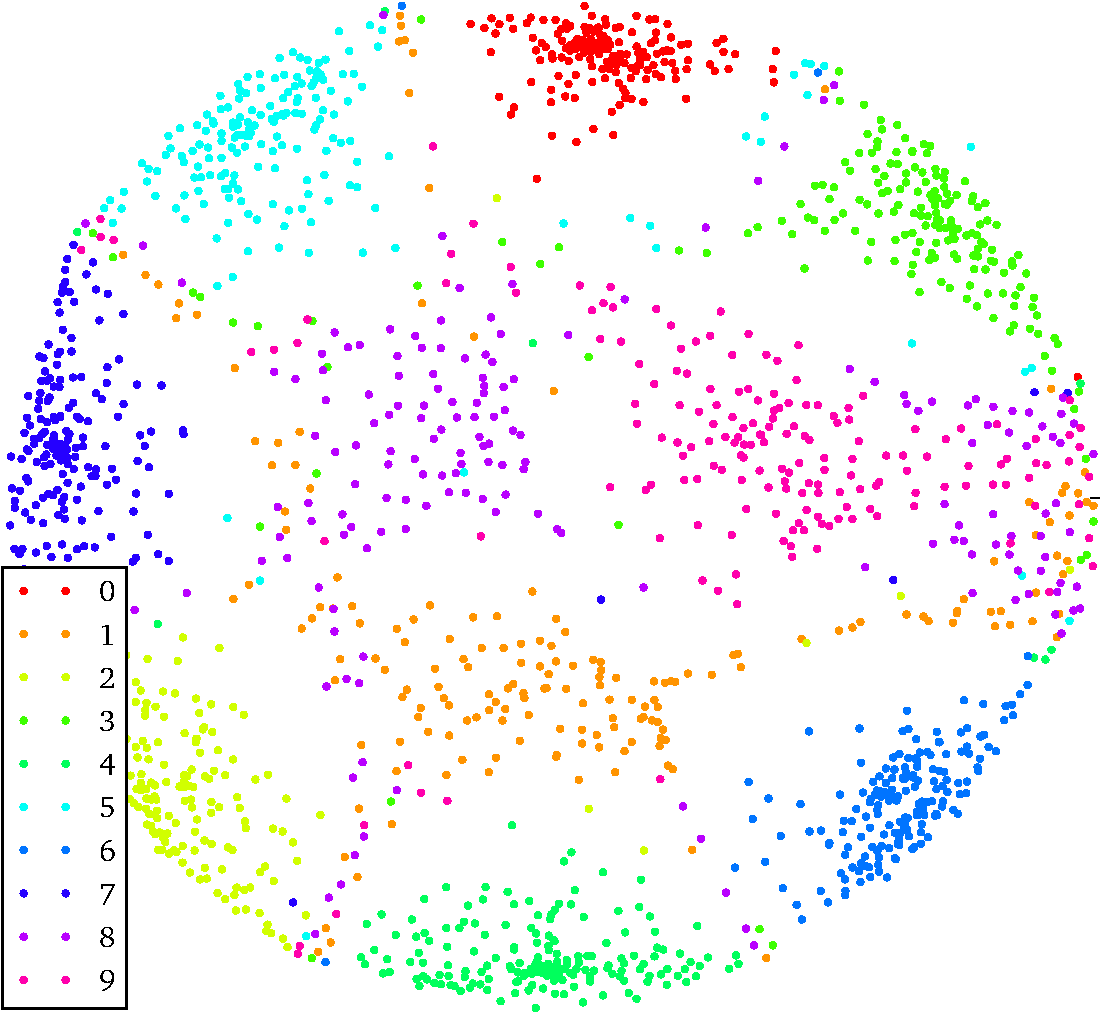
\includegraphics[width=0.9\textwidth]{figures/ch4_proximity_plot.pdf}
    \caption{Proximity plot for a 10-class handwritten digit classification task.}
    \label{fig:proximity-plot}
\end{figure}

For exploratory purposes, the $N\times N$ proximity matrix $P$ such that
\begin{equation}
P_{ij} = \text{proximity}(\mathbf{x}_i, \mathbf{x}_j),
\end{equation}
can be used to visually represent how samples are close together with respect
to the random forest. Using $1-P$ as a dissimilarity matrix,  the level of
similarity between individual samples can be visualized e.g., by projecting them
on a $d$-dimensional space (e.g., on a plane) such that the distances
between any pair of samples in that space correspond as best as possible to the
dissimilarities in $1-P$. As an illustrative example, Figure~\ref{fig:proximity-plot}
represents the proximity matrix learned for a 10-class handwritten digit
classification task, as projected on a plane using Multidimensional Scaling~\citep{kruskal:1964}.
Samples from a same class form identifiable clusters, which suggests that
they share similar structure (since they end up in the same leaves). The figure
also highlights classes for which the random forest makes errors. In this case,
digits $1$ and $8$ are the more dispersed, suggesting high within-class variance,
but also overlap the most with samples of other classes, indicating
that the random forest fails to identify the true class for these samples.

Additionally, proximity measures can be used for identifying outliers within a
learning set ${\cal L}$. A sample $\mathbf{x}$ can be considered as an outlier
if its average proximity with respect to all other samples is small, which
indeed indicates that $\mathbf{x}$ is structurally different from the other
samples (since they do not end up in the same leaves). In the same way, in
classification, within-class outliers can be identified by computing the
average proximity of a sample with respect to all other samples of the same
class. Conversely, proximity measures can be used for identifying class
prototypes, by considering samples whose proximity with all other samples
of the same class is the largest.

An alternative formulation of proximity measures is to consider a random forest
as a mapping $\phi: {\cal X} \mapsto {\cal X}^\prime$ which transforms a sample
$\mathbf{x}$ into the (one-hot-encoded) indices of the leaves it ends up in.
That is, $\mathbf{x}^\prime_t$ is $1$ for all leaves $t$ of the forest in which
$\mathbf{x}$ falls in, and $0$ for all the others:
\begin{equation}
\phi(\mathbf{x}) = \Big( 1(\mathbf{x} \in {\cal X}_{t_1}), \dots, 1(\mathbf{x} \in {\cal X}_{t_L} ) \Big)
\end{equation}
where $t_1, \dots, t_L \in \widetilde{\psi}$ denote the leafs of all $M$ trees in the forest $\psi$.
In this formalism, the
proximity between $\mathbf{x}_1$ and $\mathbf{x}_2$ corresponds to a
\textit{kernel}~\citep{scholkopf:2001}\label{ntn:kernel2}, that can be defined as the normalized
dot product of the samples, as represented in ${\cal X}^\prime$:
\begin{equation}
\text{proximity}(\mathbf{x}_1, \mathbf{x}_2) = \frac{1}{M} \phi(\mathbf{x}_1) \cdot \phi(\mathbf{x}_2)
\end{equation}
Interestingly, $\phi$ provides a non-linear transformation to a sparse very
high-dimensional space, taking somehow into account the structure of the
problem. If two samples are structurally similar, then they will end up in the
same leafs and their representations in the projected space will be close, even
if they may in fact appear quite dissimilar in the original space.

In close connection, \citep{geurts:2006} show that a regression tree
$\varphi$ can be expressed as a kernel-based model by formulating the
prediction $\varphi(\mathbf{x})$ as a scalar product over the input space
defined by the normalized characteristic function $\phi^\prime$ of the leaf nodes. That is,
\begin{equation}
\varphi(\mathbf{x}) = \sum_{(\mathbf{x}_i, y_i) \in {\cal L}} y_i K_\varphi(\mathbf{x}_i, \mathbf{x})
\end{equation}
where
\begin{align}
K_\varphi(\mathbf{x}_i, \mathbf{x}) &= \phi^\prime(\mathbf{x}_i) \cdot \phi^\prime(\mathbf{x}), \\
\phi^\prime(\mathbf{x}) &= \Big( \frac{1(\mathbf{x} \in {\cal X}_1)}{\sqrt{N_1}}, \dots, \frac{1(\mathbf{x} \in {\cal X}_{t_L})}{\sqrt{N_{t_L}}}  \Big),
\end{align}
and where $t_1,\dots,t_L \in \widetilde{\varphi}$ denote the leafs of $\varphi$.
Likewise, the formulation can be extended to an ensemble $\psi$ of $M$ decision
trees by defining $K_\psi$ as the average kernel over $K_{\varphi_m}$ (for $m=1,\dots,M$).

From a more practical point of view, such forest-based transforms $\phi$ and
$\phi^\prime$ have proven to be helpful and efficient embeddings, e.g., when
combined with linear methods or support vector machines
\citep{moosmann:2006,maree:2013}. In particular, they find useful applications
in computer vision for transforming the raw pixel input space into a new
feature space hopefully capturing structures and patterns in images.

\subsection{Missing data}

Because of practical limitations, physical constraints or for privacy reasons,
real-world data are often imperfect, erroneous or incomplete. In particular,
most machine learning algorithms are often not applicable on data containing
missing values because they implicitly assume an ideal scenario in which all
values are known for all input variables. Fortunately, random forests offer
several mechanisms for dealing with this issue.

\begin{description}

\item \textit{Ternary decision trees.}\hfill\\
    The simplest strategy is to explicitly model missing values in the
    structure of decision trees by considering ternary splits instead of binary
    splits. That is, partition $t$ into $t_L$, $t_R$ and $t_M$, such that $t_L$
    and $t_R$ are defined from a binary split $s_j^v : X_j \leq v$, for all node
    samples where the value of $X_j$ is known, and such that $t_M$ contain all node
    samples for which the value of $X_j$ is missing.

\item \textit{Propagate in both child nodes}\hfill\\
    An alternative strategy is to  propagate samples
    for which the value of the split variable is missing into both the left and
    right child nodes. Accordingly, samples going into both child nodes should be
    re-weighted by half their sample weight (see Chapter~\ref{ch:complexity}), so
    that they are not unfairly taken into account more than the other samples.

\item \textit{Imputation.}\hfill\\
    Finally, random forests also offer several mechanisms for imputing missing
    values. A simple approach, due to \citep{breiman:2002}, consists first in
    filling missing values with a rough and inaccurate approximation (e.g., the
    median). Then build a random forest on the completed data and update the
    missing values of each sample by the weighted mean value over the samples
    that are the closest (as defined by the proximity measure). The procedure
    is then repeated  until convergence, typically after $4$ to $6$ iterations.

    Alternatively, missing data imputation can be considered as a supervised
    learning problem in itself, where the response variable is the input
    variable for which values are missing. As such, the MissForest
    algorithm~\citep{stekhoven:2012} consists in iteratively building a random
    forest on the observed parts of the data in order to predict the missing
    values for a given variable.

\end{description}


\section{Consistency}
\label{sec:4:consistency}

Despite their extensive use in practice, excellent performance and relative
algorithmic simplicity, the mathematical mechanisms that drive random forests
are still not well understood. More specifically, the fundamental theoretical
question of the consistency (see definitions \ref{def:consistency} and
\ref{def:consistency-strong}) of random forests, i.e., whether convergence towards an
optimal model is guaranteed provided an infinitely large learning set, remains
an open and difficult problem. In this section, we review theoretical works
that have investigated simplified versions of the algorithm, for which the construction
procedure is often made data-independent, hence making the
theoretical analysis typically more tractable. With the hope that results
obtained for these simplified models will provide insights on the mathematical
properties of the actual algorithm, the long-term objective of this line of
research is usually to prove the consistency of the original Random Forest
algorithm \citep{breiman:2001}, hence bridging the gap between theory and
practice.

\begin{description}

\item \citet{breiman:1984}:\hfill \\
    Single decision trees are proved to be consistent, both in regression and
    classification.

    Note that these results do not extend to the Random Forest algorithm for the following reasons:
    \begin{itemize}
    \item In single decision trees, the number of samples in terminal nodes
          is let to become large, while trees in random forests are usually fully developed;
    \item Single decision trees do not make use of bootstrap sampling;
    \item The splitting strategy in single decision trees consists in selecting
          the split that maximizes the Gini criterion. By contrast, in random forests,
          the splitting strategy is randomized.
    \end{itemize}

\item \citet{zhao:2000}:\hfill\\
    One of the earliest works studying the consistency of ensembles of
    randomized trees is due to \citet{zhao:2000}. In classification, the author
    conjectures that PERT is (weakly) consistent, but establishes its strong
    consistency (Theorem 4.4.2) provided the construction of the trees stops early. More
    specifically, strong consistency is guaranteed provided:

    \begin{enumerate}
        \item Trees are grown
            infinitely deeply while forming leaves with infinitely many node samples,
            hence making empirical class proportions in terminal nodes
            converge towards their theoretical counterparts. This is guaranteed,
            e.g.,  by stopping the construction
            when $N_t < N_\text{min}^{(N)}$, such that
            $N_\text{min}^{(N)} \to 0$ and  $N\times N_\text{min}^{(N)} \to \infty$ as $N \to
            \infty$ (where $N_\text{min}^{(N)}$ is the value of the $N_\text{min}$ parameter
            for a forest grown on a learning set of size $N$);

        \item The posterior class probabilities induced by the ensemble are all
              continuous in the input space ${\cal X}$.
    \end{enumerate}

    Given the close formulations of the methods, results from \citep{zhao:2000}
    regarding PERT extend to Extremely Randomized Trees provided the posterior
    class probabilities are continuous. In Appendix F of \citep{geurts:2006},
    Extremely Randomizes Trees (for $K=1$ and $M \to \infty$) are shown
    to be a continuous piecewise multilinear function of its arguments,
    which should therefore suffice to establish the strong consistency of the method when
    trees are built totally at random.

\item \citet{breiman:2004}:\hfill\\
    In this work, consistency is studied for a simplified variant of the Random
    Forest algorithm, assuming (i) no bootstrap sampling, (ii) that variables are selected as split variables
    with probability $p(m)$ (for $m=1,\dots,p$), (iii) that splits on
    relevant variables are set at the midpoint of the values of the selected
    variable, (iv) that splits on irrelevant variables are set at random points
    along the values of the selected variable and (v) that trees are balanced.
    Under these assumptions,  it can be shown that this variant reduces
    to an (adaptive) nearest neighbor algorithm~\citep{lin:2006}, for which (weak) consistency
    conditions are met (both in regression and classification).
    Additionally, this work studies the bias-variance decomposition of this simplified
    method and shows that the rate of convergence towards the Bayes error
    only depends on the number $r$ of relevant variables, hence explaining
    why random forests work well even with many noise variables.

\item \citet{biau:2008}:\hfill\\
    In binary classification, \citet{biau:2008} proves that if the randomized base
    models in an ensemble are consistent, then the corresponding majority
    or soft voting ensembles are also consistent. (This result
    was later expanded both for multi-class classification~\citep{denil:2013b} and
    regression~\citep{denil:2013}.)

    From this proposition, the consistency of Purely Random Forests
    \citep{breiman2000some} is established.  Let us assume that the input space
    ${\cal X}$ is supported on $[0,1]^p$ and that terminal nodes represent
    hyper rectangles of $[0,1]^p$, called cells, and forming together a
    partition of $[0,1]^p$. At each step, one of the current terminal nodes $t$
    and one the $p$ input variables are chosen uniformly at random. The
    selected node $t$ is then split along the chosen variable at a random
    location, along the length of the chosen side in $t$. This
    procedure is repeated $k \geq 1$ times, which amounts to developing  trees
    in random order.  In this setting, and similarly to PERT, (strong) consistency of
    Purely Random Forests is guaranteed whenever $\smash{k^{(N)} \to \infty}$ and
    $\smash{\tfrac{k^{(N)}}{N} \to 0}$ as $N \to \infty$ (where $\smash{k^{(N)}}$  is the value
    of $k$ for a forest grown on learning set of size $N$) -- which is equivalent
    to letting the number of points in terminal nodes grow to infinity.

    In Purely Random Forests, let us remark that trees are built in a
    data-independent manner, without even looking at the samples in ${\cal L}$. In
    this same work, and assuming no bootstrap sampling, the authors show that consistency is however
    also guaranteed when the position of the cut is chosen in a data-dependent
    manner, by selecting a random gap between consecutive node samples (ordered
    along the chosen variable) and then sampling uniformly within the gap.

\item \citet{biau:2012}:\hfill \\
    In this work, the authors more closely approaches the consistency of the
    actual Random Forest algorithm and prove the consistency of the following
    variant.

    Again, let us assume that the input space ${\cal X}$ is supported on
    $[0,1]^p$ and that terminal nodes represent hyper rectangles of $[0,1]^p$,
    forming together a partition of the input space. At each step, all current
    terminal nodes are independently split using one of the $p$ input variables
    $X_j$, drawn with probability $p_{j}^{(N)}$, and using as threshold the
    mid-point of the chosen side in $t$. This procedure is repeated $\lceil
    \log_2 k \rceil$ times, which amounts to developing trees in breadth-first
    order until depth $\lceil \log_2 k \rceil$. (Strong) Consistency is then guaranteed
    whenever  $\smash{p_j^{(N)} k^{(N)} \to \infty}$ (for $j=1,\dots,p$) and
    $\smash{\tfrac{k^{(N)}}{N} \to 0}$ as $N \to \infty$.

    In particular, by properly defining the probabilities  $p_j$, this result
    can be shown to include the situation where, at each node, randomness is
    introduced by selecting at random a subset of $K$ variables and splitting
    along the one that maximizes some impurity criterion, like in Random
    Forest. (Note however that best cut-points coincide with the mid-points
    only for some probability distributions.) Assuming no bootstrap sampling
    and provided that two independent datasets are used for evaluating the
    goodness of the splits and fitting the prediction values at leafs,
    consistency of the method is then also established.

    Interestingly, and corroborating results of \citep{breiman:2004}, this work
    also highlights the fact that performance of random forests only depends on
    the number $r$ of relevant variables, and not on $p$, making the method
    robust to overfitting.

\item \citet{denil:2013}:\hfill \\
    Building upon \citep{biau:2012}, \citet{denil:2013} narrowed the gap
    between theory and practice by proving the consistency of the following variant.

    For each tree in the forest, the learning set is partitioned randomly into
    structure points (used for determining splits) and estimation points (used
    for fitting values at leafs).  Again, let us assume that the input space
    ${\cal X}$ is supported on $[0,1]^p$ and that terminal nodes represent
    hyper rectangles of $[0,1]^p$, forming together a partition of the input
    space. At each step, current terminal nodes are expanded by drawing at
    random $\min(1+\text{Poisson}(\lambda), p)$ variables and then looking for
    the cut-point that maximizes the impurity criterion, as computed over $m$
    randomly drawn structure points. The construction halts when no split
    leading to child nodes with less than $k$ node samples can be found.

    In regression, assuming not bootstrap sampling, (strong)  consistency of this variant
    is guaranteed whenever $k^{(N)} \to \infty$ and $\tfrac{k^{(N)}}{N} \to 0$
    as $N \to \infty$ (where $k^{(N)}$  is the value of $k$ for a forest grown
    on learning set of size $N$).

\item \citet{scornet:2014}:\hfill \\
    This work establishes the first consistency result for the original Random
    Forest algorithm. In particular, (strong)  consistency is obtained in the context of
    regression additive models, assuming subsampling without replacement
    (instead of bootstrap sampling). This work is the first result
    establishing consistency when (i) splits are chosen in a data-dependent
    manner and (ii) leafs are not let to grow to an infinite number of node samples.

\end{description}

In conclusions, despite the difficulty of the mathematical analysis of the
method, these theoretical works provide together converging arguments all
confirming why random forests -- including the Random Forest algorithm but also
Extremely Randomized Trees -- appear to work so well in practice.

Finally, let us complete this review by mentioning consistency results in the
case of domain-specific adaptations of random forests, including quantile
regression~\citep{meinshausen:2006}, survival analysis~\citep{ishwaran:2010}
and online forest construction~\citep{denil:2013b}.
